
% Default to the notebook output style

    


% Inherit from the specified cell style.




    
\documentclass[11pt]{article}

    
    
    \usepackage[T1]{fontenc}
    % Nicer default font (+ math font) than Computer Modern for most use cases
    \usepackage{mathpazo}

    % Basic figure setup, for now with no caption control since it's done
    % automatically by Pandoc (which extracts ![](path) syntax from Markdown).
    \usepackage{graphicx}
    % We will generate all images so they have a width \maxwidth. This means
    % that they will get their normal width if they fit onto the page, but
    % are scaled down if they would overflow the margins.
    \makeatletter
    \def\maxwidth{\ifdim\Gin@nat@width>\linewidth\linewidth
    \else\Gin@nat@width\fi}
    \makeatother
    \let\Oldincludegraphics\includegraphics
    % Set max figure width to be 80% of text width, for now hardcoded.
    \renewcommand{\includegraphics}[1]{\Oldincludegraphics[width=.8\maxwidth]{#1}}
    % Ensure that by default, figures have no caption (until we provide a
    % proper Figure object with a Caption API and a way to capture that
    % in the conversion process - todo).
    \usepackage{caption}
    \DeclareCaptionLabelFormat{nolabel}{}
    \captionsetup{labelformat=nolabel}

    \usepackage{adjustbox} % Used to constrain images to a maximum size 
    \usepackage{xcolor} % Allow colors to be defined
    \usepackage{enumerate} % Needed for markdown enumerations to work
    \usepackage{geometry} % Used to adjust the document margins
    \usepackage{amsmath} % Equations
    \usepackage{amssymb} % Equations
    \usepackage{textcomp} % defines textquotesingle
    % Hack from http://tex.stackexchange.com/a/47451/13684:
    \AtBeginDocument{%
        \def\PYZsq{\textquotesingle}% Upright quotes in Pygmentized code
    }
    \usepackage{upquote} % Upright quotes for verbatim code
    \usepackage{eurosym} % defines \euro
    \usepackage[mathletters]{ucs} % Extended unicode (utf-8) support
    \usepackage[utf8x]{inputenc} % Allow utf-8 characters in the tex document
    \usepackage{fancyvrb} % verbatim replacement that allows latex
    \usepackage{grffile} % extends the file name processing of package graphics 
                         % to support a larger range 
    % The hyperref package gives us a pdf with properly built
    % internal navigation ('pdf bookmarks' for the table of contents,
    % internal cross-reference links, web links for URLs, etc.)
    \usepackage{hyperref}
    \usepackage{longtable} % longtable support required by pandoc >1.10
    \usepackage{booktabs}  % table support for pandoc > 1.12.2
    \usepackage[inline]{enumitem} % IRkernel/repr support (it uses the enumerate* environment)
    \usepackage[normalem]{ulem} % ulem is needed to support strikethroughs (\sout)
                                % normalem makes italics be italics, not underlines
    

    
    
    % Colors for the hyperref package
    \definecolor{urlcolor}{rgb}{0,.145,.698}
    \definecolor{linkcolor}{rgb}{.71,0.21,0.01}
    \definecolor{citecolor}{rgb}{.12,.54,.11}

    % ANSI colors
    \definecolor{ansi-black}{HTML}{3E424D}
    \definecolor{ansi-black-intense}{HTML}{282C36}
    \definecolor{ansi-red}{HTML}{E75C58}
    \definecolor{ansi-red-intense}{HTML}{B22B31}
    \definecolor{ansi-green}{HTML}{00A250}
    \definecolor{ansi-green-intense}{HTML}{007427}
    \definecolor{ansi-yellow}{HTML}{DDB62B}
    \definecolor{ansi-yellow-intense}{HTML}{B27D12}
    \definecolor{ansi-blue}{HTML}{208FFB}
    \definecolor{ansi-blue-intense}{HTML}{0065CA}
    \definecolor{ansi-magenta}{HTML}{D160C4}
    \definecolor{ansi-magenta-intense}{HTML}{A03196}
    \definecolor{ansi-cyan}{HTML}{60C6C8}
    \definecolor{ansi-cyan-intense}{HTML}{258F8F}
    \definecolor{ansi-white}{HTML}{C5C1B4}
    \definecolor{ansi-white-intense}{HTML}{A1A6B2}

    % commands and environments needed by pandoc snippets
    % extracted from the output of `pandoc -s`
    \providecommand{\tightlist}{%
      \setlength{\itemsep}{0pt}\setlength{\parskip}{0pt}}
    \DefineVerbatimEnvironment{Highlighting}{Verbatim}{commandchars=\\\{\}}
    % Add ',fontsize=\small' for more characters per line
    \newenvironment{Shaded}{}{}
    \newcommand{\KeywordTok}[1]{\textcolor[rgb]{0.00,0.44,0.13}{\textbf{{#1}}}}
    \newcommand{\DataTypeTok}[1]{\textcolor[rgb]{0.56,0.13,0.00}{{#1}}}
    \newcommand{\DecValTok}[1]{\textcolor[rgb]{0.25,0.63,0.44}{{#1}}}
    \newcommand{\BaseNTok}[1]{\textcolor[rgb]{0.25,0.63,0.44}{{#1}}}
    \newcommand{\FloatTok}[1]{\textcolor[rgb]{0.25,0.63,0.44}{{#1}}}
    \newcommand{\CharTok}[1]{\textcolor[rgb]{0.25,0.44,0.63}{{#1}}}
    \newcommand{\StringTok}[1]{\textcolor[rgb]{0.25,0.44,0.63}{{#1}}}
    \newcommand{\CommentTok}[1]{\textcolor[rgb]{0.38,0.63,0.69}{\textit{{#1}}}}
    \newcommand{\OtherTok}[1]{\textcolor[rgb]{0.00,0.44,0.13}{{#1}}}
    \newcommand{\AlertTok}[1]{\textcolor[rgb]{1.00,0.00,0.00}{\textbf{{#1}}}}
    \newcommand{\FunctionTok}[1]{\textcolor[rgb]{0.02,0.16,0.49}{{#1}}}
    \newcommand{\RegionMarkerTok}[1]{{#1}}
    \newcommand{\ErrorTok}[1]{\textcolor[rgb]{1.00,0.00,0.00}{\textbf{{#1}}}}
    \newcommand{\NormalTok}[1]{{#1}}
    
    % Additional commands for more recent versions of Pandoc
    \newcommand{\ConstantTok}[1]{\textcolor[rgb]{0.53,0.00,0.00}{{#1}}}
    \newcommand{\SpecialCharTok}[1]{\textcolor[rgb]{0.25,0.44,0.63}{{#1}}}
    \newcommand{\VerbatimStringTok}[1]{\textcolor[rgb]{0.25,0.44,0.63}{{#1}}}
    \newcommand{\SpecialStringTok}[1]{\textcolor[rgb]{0.73,0.40,0.53}{{#1}}}
    \newcommand{\ImportTok}[1]{{#1}}
    \newcommand{\DocumentationTok}[1]{\textcolor[rgb]{0.73,0.13,0.13}{\textit{{#1}}}}
    \newcommand{\AnnotationTok}[1]{\textcolor[rgb]{0.38,0.63,0.69}{\textbf{\textit{{#1}}}}}
    \newcommand{\CommentVarTok}[1]{\textcolor[rgb]{0.38,0.63,0.69}{\textbf{\textit{{#1}}}}}
    \newcommand{\VariableTok}[1]{\textcolor[rgb]{0.10,0.09,0.49}{{#1}}}
    \newcommand{\ControlFlowTok}[1]{\textcolor[rgb]{0.00,0.44,0.13}{\textbf{{#1}}}}
    \newcommand{\OperatorTok}[1]{\textcolor[rgb]{0.40,0.40,0.40}{{#1}}}
    \newcommand{\BuiltInTok}[1]{{#1}}
    \newcommand{\ExtensionTok}[1]{{#1}}
    \newcommand{\PreprocessorTok}[1]{\textcolor[rgb]{0.74,0.48,0.00}{{#1}}}
    \newcommand{\AttributeTok}[1]{\textcolor[rgb]{0.49,0.56,0.16}{{#1}}}
    \newcommand{\InformationTok}[1]{\textcolor[rgb]{0.38,0.63,0.69}{\textbf{\textit{{#1}}}}}
    \newcommand{\WarningTok}[1]{\textcolor[rgb]{0.38,0.63,0.69}{\textbf{\textit{{#1}}}}}
    
    
    % Define a nice break command that doesn't care if a line doesn't already
    % exist.
    \def\br{\hspace*{\fill} \\* }
    % Math Jax compatability definitions
    \def\gt{>}
    \def\lt{<}
    % Document parameters
    \title{Shell\_Dna\_EnergyLoad}
    
    
    

    % Pygments definitions
    
\makeatletter
\def\PY@reset{\let\PY@it=\relax \let\PY@bf=\relax%
    \let\PY@ul=\relax \let\PY@tc=\relax%
    \let\PY@bc=\relax \let\PY@ff=\relax}
\def\PY@tok#1{\csname PY@tok@#1\endcsname}
\def\PY@toks#1+{\ifx\relax#1\empty\else%
    \PY@tok{#1}\expandafter\PY@toks\fi}
\def\PY@do#1{\PY@bc{\PY@tc{\PY@ul{%
    \PY@it{\PY@bf{\PY@ff{#1}}}}}}}
\def\PY#1#2{\PY@reset\PY@toks#1+\relax+\PY@do{#2}}

\expandafter\def\csname PY@tok@w\endcsname{\def\PY@tc##1{\textcolor[rgb]{0.73,0.73,0.73}{##1}}}
\expandafter\def\csname PY@tok@c\endcsname{\let\PY@it=\textit\def\PY@tc##1{\textcolor[rgb]{0.25,0.50,0.50}{##1}}}
\expandafter\def\csname PY@tok@cp\endcsname{\def\PY@tc##1{\textcolor[rgb]{0.74,0.48,0.00}{##1}}}
\expandafter\def\csname PY@tok@k\endcsname{\let\PY@bf=\textbf\def\PY@tc##1{\textcolor[rgb]{0.00,0.50,0.00}{##1}}}
\expandafter\def\csname PY@tok@kp\endcsname{\def\PY@tc##1{\textcolor[rgb]{0.00,0.50,0.00}{##1}}}
\expandafter\def\csname PY@tok@kt\endcsname{\def\PY@tc##1{\textcolor[rgb]{0.69,0.00,0.25}{##1}}}
\expandafter\def\csname PY@tok@o\endcsname{\def\PY@tc##1{\textcolor[rgb]{0.40,0.40,0.40}{##1}}}
\expandafter\def\csname PY@tok@ow\endcsname{\let\PY@bf=\textbf\def\PY@tc##1{\textcolor[rgb]{0.67,0.13,1.00}{##1}}}
\expandafter\def\csname PY@tok@nb\endcsname{\def\PY@tc##1{\textcolor[rgb]{0.00,0.50,0.00}{##1}}}
\expandafter\def\csname PY@tok@nf\endcsname{\def\PY@tc##1{\textcolor[rgb]{0.00,0.00,1.00}{##1}}}
\expandafter\def\csname PY@tok@nc\endcsname{\let\PY@bf=\textbf\def\PY@tc##1{\textcolor[rgb]{0.00,0.00,1.00}{##1}}}
\expandafter\def\csname PY@tok@nn\endcsname{\let\PY@bf=\textbf\def\PY@tc##1{\textcolor[rgb]{0.00,0.00,1.00}{##1}}}
\expandafter\def\csname PY@tok@ne\endcsname{\let\PY@bf=\textbf\def\PY@tc##1{\textcolor[rgb]{0.82,0.25,0.23}{##1}}}
\expandafter\def\csname PY@tok@nv\endcsname{\def\PY@tc##1{\textcolor[rgb]{0.10,0.09,0.49}{##1}}}
\expandafter\def\csname PY@tok@no\endcsname{\def\PY@tc##1{\textcolor[rgb]{0.53,0.00,0.00}{##1}}}
\expandafter\def\csname PY@tok@nl\endcsname{\def\PY@tc##1{\textcolor[rgb]{0.63,0.63,0.00}{##1}}}
\expandafter\def\csname PY@tok@ni\endcsname{\let\PY@bf=\textbf\def\PY@tc##1{\textcolor[rgb]{0.60,0.60,0.60}{##1}}}
\expandafter\def\csname PY@tok@na\endcsname{\def\PY@tc##1{\textcolor[rgb]{0.49,0.56,0.16}{##1}}}
\expandafter\def\csname PY@tok@nt\endcsname{\let\PY@bf=\textbf\def\PY@tc##1{\textcolor[rgb]{0.00,0.50,0.00}{##1}}}
\expandafter\def\csname PY@tok@nd\endcsname{\def\PY@tc##1{\textcolor[rgb]{0.67,0.13,1.00}{##1}}}
\expandafter\def\csname PY@tok@s\endcsname{\def\PY@tc##1{\textcolor[rgb]{0.73,0.13,0.13}{##1}}}
\expandafter\def\csname PY@tok@sd\endcsname{\let\PY@it=\textit\def\PY@tc##1{\textcolor[rgb]{0.73,0.13,0.13}{##1}}}
\expandafter\def\csname PY@tok@si\endcsname{\let\PY@bf=\textbf\def\PY@tc##1{\textcolor[rgb]{0.73,0.40,0.53}{##1}}}
\expandafter\def\csname PY@tok@se\endcsname{\let\PY@bf=\textbf\def\PY@tc##1{\textcolor[rgb]{0.73,0.40,0.13}{##1}}}
\expandafter\def\csname PY@tok@sr\endcsname{\def\PY@tc##1{\textcolor[rgb]{0.73,0.40,0.53}{##1}}}
\expandafter\def\csname PY@tok@ss\endcsname{\def\PY@tc##1{\textcolor[rgb]{0.10,0.09,0.49}{##1}}}
\expandafter\def\csname PY@tok@sx\endcsname{\def\PY@tc##1{\textcolor[rgb]{0.00,0.50,0.00}{##1}}}
\expandafter\def\csname PY@tok@m\endcsname{\def\PY@tc##1{\textcolor[rgb]{0.40,0.40,0.40}{##1}}}
\expandafter\def\csname PY@tok@gh\endcsname{\let\PY@bf=\textbf\def\PY@tc##1{\textcolor[rgb]{0.00,0.00,0.50}{##1}}}
\expandafter\def\csname PY@tok@gu\endcsname{\let\PY@bf=\textbf\def\PY@tc##1{\textcolor[rgb]{0.50,0.00,0.50}{##1}}}
\expandafter\def\csname PY@tok@gd\endcsname{\def\PY@tc##1{\textcolor[rgb]{0.63,0.00,0.00}{##1}}}
\expandafter\def\csname PY@tok@gi\endcsname{\def\PY@tc##1{\textcolor[rgb]{0.00,0.63,0.00}{##1}}}
\expandafter\def\csname PY@tok@gr\endcsname{\def\PY@tc##1{\textcolor[rgb]{1.00,0.00,0.00}{##1}}}
\expandafter\def\csname PY@tok@ge\endcsname{\let\PY@it=\textit}
\expandafter\def\csname PY@tok@gs\endcsname{\let\PY@bf=\textbf}
\expandafter\def\csname PY@tok@gp\endcsname{\let\PY@bf=\textbf\def\PY@tc##1{\textcolor[rgb]{0.00,0.00,0.50}{##1}}}
\expandafter\def\csname PY@tok@go\endcsname{\def\PY@tc##1{\textcolor[rgb]{0.53,0.53,0.53}{##1}}}
\expandafter\def\csname PY@tok@gt\endcsname{\def\PY@tc##1{\textcolor[rgb]{0.00,0.27,0.87}{##1}}}
\expandafter\def\csname PY@tok@err\endcsname{\def\PY@bc##1{\setlength{\fboxsep}{0pt}\fcolorbox[rgb]{1.00,0.00,0.00}{1,1,1}{\strut ##1}}}
\expandafter\def\csname PY@tok@kc\endcsname{\let\PY@bf=\textbf\def\PY@tc##1{\textcolor[rgb]{0.00,0.50,0.00}{##1}}}
\expandafter\def\csname PY@tok@kd\endcsname{\let\PY@bf=\textbf\def\PY@tc##1{\textcolor[rgb]{0.00,0.50,0.00}{##1}}}
\expandafter\def\csname PY@tok@kn\endcsname{\let\PY@bf=\textbf\def\PY@tc##1{\textcolor[rgb]{0.00,0.50,0.00}{##1}}}
\expandafter\def\csname PY@tok@kr\endcsname{\let\PY@bf=\textbf\def\PY@tc##1{\textcolor[rgb]{0.00,0.50,0.00}{##1}}}
\expandafter\def\csname PY@tok@bp\endcsname{\def\PY@tc##1{\textcolor[rgb]{0.00,0.50,0.00}{##1}}}
\expandafter\def\csname PY@tok@fm\endcsname{\def\PY@tc##1{\textcolor[rgb]{0.00,0.00,1.00}{##1}}}
\expandafter\def\csname PY@tok@vc\endcsname{\def\PY@tc##1{\textcolor[rgb]{0.10,0.09,0.49}{##1}}}
\expandafter\def\csname PY@tok@vg\endcsname{\def\PY@tc##1{\textcolor[rgb]{0.10,0.09,0.49}{##1}}}
\expandafter\def\csname PY@tok@vi\endcsname{\def\PY@tc##1{\textcolor[rgb]{0.10,0.09,0.49}{##1}}}
\expandafter\def\csname PY@tok@vm\endcsname{\def\PY@tc##1{\textcolor[rgb]{0.10,0.09,0.49}{##1}}}
\expandafter\def\csname PY@tok@sa\endcsname{\def\PY@tc##1{\textcolor[rgb]{0.73,0.13,0.13}{##1}}}
\expandafter\def\csname PY@tok@sb\endcsname{\def\PY@tc##1{\textcolor[rgb]{0.73,0.13,0.13}{##1}}}
\expandafter\def\csname PY@tok@sc\endcsname{\def\PY@tc##1{\textcolor[rgb]{0.73,0.13,0.13}{##1}}}
\expandafter\def\csname PY@tok@dl\endcsname{\def\PY@tc##1{\textcolor[rgb]{0.73,0.13,0.13}{##1}}}
\expandafter\def\csname PY@tok@s2\endcsname{\def\PY@tc##1{\textcolor[rgb]{0.73,0.13,0.13}{##1}}}
\expandafter\def\csname PY@tok@sh\endcsname{\def\PY@tc##1{\textcolor[rgb]{0.73,0.13,0.13}{##1}}}
\expandafter\def\csname PY@tok@s1\endcsname{\def\PY@tc##1{\textcolor[rgb]{0.73,0.13,0.13}{##1}}}
\expandafter\def\csname PY@tok@mb\endcsname{\def\PY@tc##1{\textcolor[rgb]{0.40,0.40,0.40}{##1}}}
\expandafter\def\csname PY@tok@mf\endcsname{\def\PY@tc##1{\textcolor[rgb]{0.40,0.40,0.40}{##1}}}
\expandafter\def\csname PY@tok@mh\endcsname{\def\PY@tc##1{\textcolor[rgb]{0.40,0.40,0.40}{##1}}}
\expandafter\def\csname PY@tok@mi\endcsname{\def\PY@tc##1{\textcolor[rgb]{0.40,0.40,0.40}{##1}}}
\expandafter\def\csname PY@tok@il\endcsname{\def\PY@tc##1{\textcolor[rgb]{0.40,0.40,0.40}{##1}}}
\expandafter\def\csname PY@tok@mo\endcsname{\def\PY@tc##1{\textcolor[rgb]{0.40,0.40,0.40}{##1}}}
\expandafter\def\csname PY@tok@ch\endcsname{\let\PY@it=\textit\def\PY@tc##1{\textcolor[rgb]{0.25,0.50,0.50}{##1}}}
\expandafter\def\csname PY@tok@cm\endcsname{\let\PY@it=\textit\def\PY@tc##1{\textcolor[rgb]{0.25,0.50,0.50}{##1}}}
\expandafter\def\csname PY@tok@cpf\endcsname{\let\PY@it=\textit\def\PY@tc##1{\textcolor[rgb]{0.25,0.50,0.50}{##1}}}
\expandafter\def\csname PY@tok@c1\endcsname{\let\PY@it=\textit\def\PY@tc##1{\textcolor[rgb]{0.25,0.50,0.50}{##1}}}
\expandafter\def\csname PY@tok@cs\endcsname{\let\PY@it=\textit\def\PY@tc##1{\textcolor[rgb]{0.25,0.50,0.50}{##1}}}

\def\PYZbs{\char`\\}
\def\PYZus{\char`\_}
\def\PYZob{\char`\{}
\def\PYZcb{\char`\}}
\def\PYZca{\char`\^}
\def\PYZam{\char`\&}
\def\PYZlt{\char`\<}
\def\PYZgt{\char`\>}
\def\PYZsh{\char`\#}
\def\PYZpc{\char`\%}
\def\PYZdl{\char`\$}
\def\PYZhy{\char`\-}
\def\PYZsq{\char`\'}
\def\PYZdq{\char`\"}
\def\PYZti{\char`\~}
% for compatibility with earlier versions
\def\PYZat{@}
\def\PYZlb{[}
\def\PYZrb{]}
\makeatother


    % Exact colors from NB
    \definecolor{incolor}{rgb}{0.0, 0.0, 0.5}
    \definecolor{outcolor}{rgb}{0.545, 0.0, 0.0}



    
    % Prevent overflowing lines due to hard-to-break entities
    \sloppy 
    % Setup hyperref package
    \hypersetup{
      breaklinks=true,  % so long urls are correctly broken across lines
      colorlinks=true,
      urlcolor=urlcolor,
      linkcolor=linkcolor,
      citecolor=citecolor,
      }
    % Slightly bigger margins than the latex defaults
    
    \geometry{verbose,tmargin=1in,bmargin=1in,lmargin=1in,rmargin=1in}
    
    

    \begin{document}
    
    
    \maketitle
    
    

    
    \section{Shell APD Learning eXchange DnA
Notebook}\label{shell-apd-learning-exchange-dna-notebook}

\subsection{Predicting power usage in the eastern United
States}\label{predicting-power-usage-in-the-eastern-united-states}

In this notebook, we will go through the cycle of a typical data science
project, starting with data collection, cleaning, feature engineering
and finally predictive modeling. We will also explore the three
different categories of machine learning problems, and how they work. By
the end of this exercise notebook you should have a basic understanding
of how data science works.

    \subsection{PJM Hourly Energy Consumption
Data}\label{pjm-hourly-energy-consumption-data}

PJM is a regional transmission organization in the United States. It is
part of the Eastern Interconnection grid operating an electric
transmission system serving all or parts of Delaware, Illinois, Indiana,
Kentucky, Maryland, Michigan, New Jersey, North Carolina, Ohio,
Pennsylvania, Tennessee, Virginia, West Virginia, and the District of
Columbia.

We will be using hourly power consumption data from PJM's East grid.
This data set ranges from 2002-2018. The data came from PJM's website
and are given in megawatts (MW).

    \subsection{Overview:}\label{overview}

\paragraph{Day 1}\label{day-1}

\begin{enumerate}
\def\labelenumi{\arabic{enumi}.}
\setcounter{enumi}{-1}
\tightlist
\item
  Section \ref{intro}
\item
  Section \ref{setup}
\item
  Section \ref{data}
\item
  Section \ref{explore}
\item
  Section \ref{traintest}
\item
  Section \ref{model}

  \begin{itemize}
  \tightlist
  \item
    Section \ref{linear}
  \item
    Section \ref{xgbreg}
  \end{itemize}
\end{enumerate}

\paragraph{Day 2}\label{day-2}

\begin{enumerate}
\def\labelenumi{\arabic{enumi}.}
\setcounter{enumi}{5}
\tightlist
\item
  Section \ref{featureengineer}
\item
  Section \ref{cleaning}
\item
  Section \ref{modelnew}
\item
  Section \ref{classification}\\
\item
  Section \ref{clustering}
\item
  Section \ref{nextsteps}
\end{enumerate}

\begin{longtable}[]{@{}lll@{}}
\toprule
REGRESSION & CLASSIFICATION & CLUSTERING\tabularnewline
\midrule
\endhead
& &\tabularnewline
\bottomrule
\end{longtable}

    \section{1. Import some python libraries and define functions we'll need
}\label{import-some-python-libraries-and-define-functions-well-need}

    \begin{Verbatim}[commandchars=\\\{\}]
{\color{incolor}In [{\color{incolor}1}]:} \PY{o}{\PYZpc{}\PYZpc{}}\PY{k}{capture}
        
        import numpy as np
        import pandas as pd
        import seaborn as sns
        import matplotlib.pyplot as plt
        from matplotlib import cm
        import matplotlib.dates as mdates
        import xgboost as xgb
        from xgboost import plot\PYZus{}importance, plot\PYZus{}tree
        from sklearn.metrics import mean\PYZus{}squared\PYZus{}error, mean\PYZus{}absolute\PYZus{}error, r2\PYZus{}score
        from sklearn.linear\PYZus{}model import LinearRegression, SGDClassifier
        from sklearn.ensemble import RandomForestClassifier
        from sklearn.metrics import confusion\PYZus{}matrix
        from sklearn.metrics import precision\PYZus{}score, recall\PYZus{}score
        from sklearn.metrics import f1\PYZus{}score
        from sklearn.cluster import KMeans
        import seaborn as sns
        import math
        from datetime import datetime
        
        def mean\PYZus{}absolute\PYZus{}percentage\PYZus{}error(y\PYZus{}true, y\PYZus{}pred): 
            \PYZdq{}\PYZdq{}\PYZdq{}Calculates MAPE given y\PYZus{}true and y\PYZus{}pred\PYZdq{}\PYZdq{}\PYZdq{}
            y\PYZus{}true, y\PYZus{}pred = np.array(y\PYZus{}true), np.array(y\PYZus{}pred)
            return np.mean(np.abs((y\PYZus{}true \PYZhy{} y\PYZus{}pred) / y\PYZus{}true)) * 100
        
        def plot\PYZus{}confusion\PYZus{}matrix(y\PYZus{}true, y\PYZus{}pred, classes,
                                  normalize=False,
                                  title=None,
                                  cmap=plt.cm.Blues):
            \PYZdq{}\PYZdq{}\PYZdq{}
            This function prints and plots the confusion matrix.
            Normalization can be applied by setting `normalize=True`.
            \PYZdq{}\PYZdq{}\PYZdq{}
            if not title:
                if normalize:
                    title = \PYZsq{}Normalized confusion matrix\PYZsq{}
                else:
                    title = \PYZsq{}Confusion matrix, without normalization\PYZsq{}
        
            \PYZsh{} Compute confusion matrix
            cm = confusion\PYZus{}matrix(y\PYZus{}true, y\PYZus{}pred)
            \PYZsh{} Only use the labels that appear in the data
        \PYZsh{}     classes = classes[unique\PYZus{}labels(y\PYZus{}true, y\PYZus{}pred)]
            if normalize:
                cm = cm.astype(\PYZsq{}float\PYZsq{}) / cm.sum(axis=1)[:, np.newaxis]
                print(\PYZdq{}Normalized confusion matrix\PYZdq{})
            else:
                print(\PYZsq{}Confusion matrix, without normalization\PYZsq{})
        
            print(cm)
        
            fig, ax = plt.subplots()
            im = ax.imshow(cm, interpolation=\PYZsq{}nearest\PYZsq{}, cmap=cmap)
            ax.figure.colorbar(im, ax=ax)
            \PYZsh{} We want to show all ticks...
            ax.set(xticks=np.arange(cm.shape[1]),
                   yticks=np.arange(cm.shape[0]),
                   \PYZsh{} ... and label them with the respective list entries
                   xticklabels=classes, yticklabels=classes,
                   title=title,
                   ylabel=\PYZsq{}True label\PYZsq{},
                   xlabel=\PYZsq{}Predicted label\PYZsq{})
        
            \PYZsh{} Rotate the tick labels and set their alignment.
            plt.setp(ax.get\PYZus{}xticklabels(), rotation=45, ha=\PYZdq{}right\PYZdq{},
                     rotation\PYZus{}mode=\PYZdq{}anchor\PYZdq{})
        
            \PYZsh{} Loop over data dimensions and create text annotations.
            fmt = \PYZsq{}.2f\PYZsq{} if normalize else \PYZsq{}d\PYZsq{}
            thresh = cm.max() / 2.
            for i in range(cm.shape[0]):
                for j in range(cm.shape[1]):
                    ax.text(j, i, format(cm[i, j], fmt),
                            ha=\PYZdq{}center\PYZdq{}, va=\PYZdq{}center\PYZdq{},
                            color=\PYZdq{}white\PYZdq{} if cm[i, j] \PYZgt{} thresh else \PYZdq{}black\PYZdq{})
            fig.tight\PYZus{}layout()
            return ax
        
        color\PYZus{}pal = [\PYZdq{}\PYZsh{}F8766D\PYZdq{}, \PYZdq{}\PYZsh{}D39200\PYZdq{}, \PYZdq{}\PYZsh{}93AA00\PYZdq{}, \PYZdq{}\PYZsh{}00BA38\PYZdq{}, \PYZdq{}\PYZsh{}00C19F\PYZdq{}, \PYZdq{}\PYZsh{}00B9E3\PYZdq{}, \PYZdq{}\PYZsh{}619CFF\PYZdq{}, \PYZdq{}\PYZsh{}DB72FB\PYZdq{}]
        
        np.set\PYZus{}printoptions(precision=2)
        pd.set\PYZus{}option(\PYZsq{}display.max\PYZus{}columns\PYZsq{}, None)
        plt.style.use(\PYZsq{}fivethirtyeight\PYZsq{})
\end{Verbatim}


    \section{2. Download the data to our notebook
}\label{download-the-data-to-our-notebook}

    \begin{Verbatim}[commandchars=\\\{\}]
{\color{incolor}In [{\color{incolor}2}]:} \PY{n}{url} \PY{o}{=} \PY{l+s+s1}{\PYZsq{}}\PY{l+s+s1}{https://github.com/robmoratore/ShellDnA/raw/master/data/PJM\PYZus{}Load.csv}\PY{l+s+s1}{\PYZsq{}}
        \PY{n}{df\PYZus{}full} \PY{o}{=} \PY{n}{pd}\PY{o}{.}\PY{n}{read\PYZus{}csv}\PY{p}{(}\PY{n}{url}\PY{p}{,} \PY{n}{sep} \PY{o}{=} \PY{l+s+s1}{\PYZsq{}}\PY{l+s+s1}{,}\PY{l+s+s1}{\PYZsq{}}\PY{p}{,} \PY{n}{date\PYZus{}parser}\PY{o}{=}\PY{p}{[}\PY{l+s+s2}{\PYZdq{}}\PY{l+s+s2}{date}\PY{l+s+s2}{\PYZdq{}}\PY{p}{]}\PY{p}{)}
        \PY{n}{df\PYZus{}full}\PY{o}{.}\PY{n}{index} \PY{o}{=} \PY{n}{pd}\PY{o}{.}\PY{n}{DatetimeIndex}\PY{p}{(}\PY{n}{df\PYZus{}full}\PY{p}{[}\PY{l+s+s2}{\PYZdq{}}\PY{l+s+s2}{date}\PY{l+s+s2}{\PYZdq{}}\PY{p}{]}\PY{p}{)}
        \PY{n}{df\PYZus{}full} \PY{o}{=} \PY{n}{df\PYZus{}full}\PY{o}{.}\PY{n}{drop}\PY{p}{(}\PY{n}{columns}\PY{o}{=}\PY{p}{[}\PY{l+s+s1}{\PYZsq{}}\PY{l+s+s1}{date}\PY{l+s+s1}{\PYZsq{}}\PY{p}{]}\PY{p}{)}
        \PY{n}{pjme} \PY{o}{=} \PY{n}{df\PYZus{}full}\PY{p}{[}\PY{p}{[}\PY{l+s+s1}{\PYZsq{}}\PY{l+s+s1}{load}\PY{l+s+s1}{\PYZsq{}}\PY{p}{,} \PY{l+s+s1}{\PYZsq{}}\PY{l+s+s1}{dayofyear}\PY{l+s+s1}{\PYZsq{}}\PY{p}{]}\PY{p}{]}
\end{Verbatim}


    \section{3. Explore the data }\label{explore-the-data}

    \subsubsection{Let's look at the first few rows of the
dataset}\label{lets-look-at-the-first-few-rows-of-the-dataset}

    \begin{Verbatim}[commandchars=\\\{\}]
{\color{incolor}In [{\color{incolor}3}]:} \PY{n}{pjme}\PY{o}{.}\PY{n}{head}\PY{p}{(}\PY{p}{)}
\end{Verbatim}


\begin{Verbatim}[commandchars=\\\{\}]
{\color{outcolor}Out[{\color{outcolor}3}]:}                       load  dayofyear
        date                                 
        2002-01-01 01:00:00  30393          1
        2002-01-01 02:00:00  29265          1
        2002-01-01 03:00:00  28357          1
        2002-01-01 04:00:00  27899          1
        2002-01-01 05:00:00  28057          1
\end{Verbatim}
            
    \subsubsection{Plot energy usage over
time}\label{plot-energy-usage-over-time}

    \begin{Verbatim}[commandchars=\\\{\}]
{\color{incolor}In [{\color{incolor}4}]:} \PY{n}{\PYZus{}} \PY{o}{=} \PY{n}{pjme}\PY{p}{[}\PY{l+s+s2}{\PYZdq{}}\PY{l+s+s2}{load}\PY{l+s+s2}{\PYZdq{}}\PY{p}{]}\PY{o}{.}\PY{n}{plot}\PY{p}{(}\PY{n}{style}\PY{o}{=}\PY{l+s+s1}{\PYZsq{}}\PY{l+s+s1}{.}\PY{l+s+s1}{\PYZsq{}}\PY{p}{,} \PY{n}{figsize}\PY{o}{=}\PY{p}{(}\PY{l+m+mi}{15}\PY{p}{,}\PY{l+m+mi}{5}\PY{p}{)}\PY{p}{,} \PY{n}{color}\PY{o}{=}\PY{n}{color\PYZus{}pal}\PY{p}{[}\PY{l+m+mi}{0}\PY{p}{]}\PY{p}{,} \PY{n}{title}\PY{o}{=}\PY{l+s+s1}{\PYZsq{}}\PY{l+s+s1}{Energy consumption}\PY{l+s+s1}{\PYZsq{}}\PY{p}{)}
        \PY{n}{\PYZus{}}\PY{o}{.}\PY{n}{set}\PY{p}{(}\PY{n}{xlabel}\PY{o}{=}\PY{l+s+s2}{\PYZdq{}}\PY{l+s+s2}{Time}\PY{l+s+s2}{\PYZdq{}}\PY{p}{,} \PY{n}{ylabel}\PY{o}{=}\PY{l+s+s2}{\PYZdq{}}\PY{l+s+s2}{Energy}\PY{l+s+s2}{\PYZdq{}}\PY{p}{)}
\end{Verbatim}


\begin{Verbatim}[commandchars=\\\{\}]
{\color{outcolor}Out[{\color{outcolor}4}]:} [Text(0,0.5,'Energy'), Text(0.5,0,'Time')]
\end{Verbatim}
            
    \begin{center}
    \adjustimage{max size={0.9\linewidth}{0.9\paperheight}}{output_11_1.png}
    \end{center}
    { \hspace*{\fill} \\}
    
    \section{4. Split the train and testing sets
}\label{split-the-train-and-testing-sets}

We do that to ensure our model is able to generalize. That means,
perform well on unseen data. If we train and test using the same data,
the model will memorize that specific output and not learn it.

We will use the data from 2015 on as our test set.

\begin{figure}
\centering
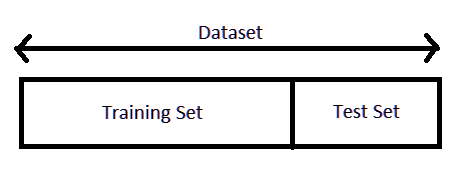
\includegraphics{https://github.com/robmoratore/ShellDnA/blob/master/data/images/train_test.png?raw=true}
\caption{alt}
\end{figure}

    \begin{Verbatim}[commandchars=\\\{\}]
{\color{incolor}In [{\color{incolor}5}]:} \PY{n}{split\PYZus{}date} \PY{o}{=} \PY{l+s+s1}{\PYZsq{}}\PY{l+s+s1}{2015\PYZhy{}01\PYZhy{}01}\PY{l+s+s1}{\PYZsq{}}
        \PY{n}{pjme\PYZus{}train} \PY{o}{=} \PY{n}{pjme}\PY{o}{.}\PY{n}{loc}\PY{p}{[}\PY{n}{pjme}\PY{o}{.}\PY{n}{index} \PY{o}{\PYZlt{}}\PY{o}{=} \PY{n}{split\PYZus{}date}\PY{p}{]}\PY{o}{.}\PY{n}{copy}\PY{p}{(}\PY{p}{)}
        \PY{n}{pjme\PYZus{}test} \PY{o}{=} \PY{n}{pjme}\PY{o}{.}\PY{n}{loc}\PY{p}{[}\PY{n}{pjme}\PY{o}{.}\PY{n}{index} \PY{o}{\PYZgt{}} \PY{n}{split\PYZus{}date}\PY{p}{]}\PY{o}{.}\PY{n}{copy}\PY{p}{(}\PY{p}{)}
\end{Verbatim}


    \begin{Verbatim}[commandchars=\\\{\}]
{\color{incolor}In [{\color{incolor}6}]:} \PY{n}{ax} \PY{o}{=} \PY{n}{pd}\PY{o}{.}\PY{n}{DataFrame}\PY{p}{(}\PY{n}{pjme\PYZus{}test}\PY{p}{[}\PY{l+s+s2}{\PYZdq{}}\PY{l+s+s2}{load}\PY{l+s+s2}{\PYZdq{}}\PY{p}{]}\PY{p}{)} \PYZbs{}
            \PY{o}{.}\PY{n}{rename}\PY{p}{(}\PY{n}{columns}\PY{o}{=}\PY{p}{\PYZob{}}\PY{l+s+s1}{\PYZsq{}}\PY{l+s+s1}{load}\PY{l+s+s1}{\PYZsq{}}\PY{p}{:} \PY{l+s+s1}{\PYZsq{}}\PY{l+s+s1}{TEST SET}\PY{l+s+s1}{\PYZsq{}}\PY{p}{\PYZcb{}}\PY{p}{)} \PYZbs{}
            \PY{o}{.}\PY{n}{join}\PY{p}{(}\PY{n}{pd}\PY{o}{.}\PY{n}{DataFrame}\PY{p}{(}\PY{n}{pjme\PYZus{}train}\PY{p}{[}\PY{l+s+s2}{\PYZdq{}}\PY{l+s+s2}{load}\PY{l+s+s2}{\PYZdq{}}\PY{p}{]}\PY{p}{)}\PY{o}{.}\PY{n}{rename}\PY{p}{(}\PY{n}{columns}\PY{o}{=}\PY{p}{\PYZob{}}\PY{l+s+s1}{\PYZsq{}}\PY{l+s+s1}{load}\PY{l+s+s1}{\PYZsq{}}\PY{p}{:} \PY{l+s+s1}{\PYZsq{}}\PY{l+s+s1}{TRAINING SET}\PY{l+s+s1}{\PYZsq{}}\PY{p}{\PYZcb{}}\PY{p}{)}\PY{p}{,} \PY{n}{how}\PY{o}{=}\PY{l+s+s1}{\PYZsq{}}\PY{l+s+s1}{outer}\PY{l+s+s1}{\PYZsq{}}\PY{p}{)} \PYZbs{}
            \PY{o}{.}\PY{n}{plot}\PY{p}{(}\PY{n}{figsize}\PY{o}{=}\PY{p}{(}\PY{l+m+mi}{15}\PY{p}{,}\PY{l+m+mi}{5}\PY{p}{)}\PY{p}{,} \PY{n}{title}\PY{o}{=}\PY{l+s+s1}{\PYZsq{}}\PY{l+s+s1}{Energy consumption}\PY{l+s+s1}{\PYZsq{}}\PY{p}{,} \PY{n}{style}\PY{o}{=}\PY{l+s+s1}{\PYZsq{}}\PY{l+s+s1}{.}\PY{l+s+s1}{\PYZsq{}}\PY{p}{)}
        
        \PY{n}{\PYZus{}} \PY{o}{=} \PY{n}{ax}\PY{o}{.}\PY{n}{set}\PY{p}{(}\PY{n}{xlabel}\PY{o}{=}\PY{l+s+s2}{\PYZdq{}}\PY{l+s+s2}{Time}\PY{l+s+s2}{\PYZdq{}}\PY{p}{,} \PY{n}{ylabel}\PY{o}{=}\PY{l+s+s2}{\PYZdq{}}\PY{l+s+s2}{Energy}\PY{l+s+s2}{\PYZdq{}}\PY{p}{)}
\end{Verbatim}


    \begin{center}
    \adjustimage{max size={0.9\linewidth}{0.9\paperheight}}{output_14_0.png}
    \end{center}
    { \hspace*{\fill} \\}
    
    \section{5. Regression - Can we predict energy use for a given hour?
}\label{regression---can-we-predict-energy-use-for-a-given-hour}

\subsection{\texorpdfstring{\[ \hat{y}(w,x) = w_0 + w_1 x_1 + w_2 x_2 + ... + w_p x_p \]}{ \textbackslash{}hat\{y\}(w,x) = w\_0 + w\_1 x\_1 + w\_2 x\_2 + ... + w\_p x\_p }}\label{hatywx-w_0-w_1-x_1-w_2-x_2-...-w_p-x_p}

    \subsection{5.1 Start with a simple model - Linear Regression
}\label{start-with-a-simple-model---linear-regression}

    \begin{Verbatim}[commandchars=\\\{\}]
{\color{incolor}In [{\color{incolor}7}]:} \PY{n}{lin\PYZus{}reg} \PY{o}{=} \PY{n}{LinearRegression}\PY{p}{(}\PY{p}{)}
        \PY{n}{lin\PYZus{}reg}\PY{o}{.}\PY{n}{fit}\PY{p}{(}\PY{n}{pjme\PYZus{}train}\PY{p}{[}\PY{l+s+s2}{\PYZdq{}}\PY{l+s+s2}{dayofyear}\PY{l+s+s2}{\PYZdq{}}\PY{p}{]}\PY{o}{.}\PY{n}{values}\PY{o}{.}\PY{n}{reshape}\PY{p}{(}\PY{o}{\PYZhy{}}\PY{l+m+mi}{1}\PY{p}{,} \PY{l+m+mi}{1}\PY{p}{)}\PY{p}{,} \PY{n}{pjme\PYZus{}train}\PY{p}{[}\PY{l+s+s2}{\PYZdq{}}\PY{l+s+s2}{load}\PY{l+s+s2}{\PYZdq{}}\PY{p}{]}\PY{o}{.}\PY{n}{values}\PY{o}{.}\PY{n}{reshape}\PY{p}{(}\PY{o}{\PYZhy{}}\PY{l+m+mi}{1}\PY{p}{,} \PY{l+m+mi}{1}\PY{p}{)}\PY{p}{)}
        \PY{n}{pjme\PYZus{}test}\PY{p}{[}\PY{l+s+s1}{\PYZsq{}}\PY{l+s+s1}{load\PYZus{}Prediction\PYZus{}lin}\PY{l+s+s1}{\PYZsq{}}\PY{p}{]} \PY{o}{=} \PY{n}{lin\PYZus{}reg}\PY{o}{.}\PY{n}{predict}\PY{p}{(}\PY{n}{pjme\PYZus{}test}\PY{p}{[}\PY{l+s+s2}{\PYZdq{}}\PY{l+s+s2}{dayofyear}\PY{l+s+s2}{\PYZdq{}}\PY{p}{]}\PY{o}{.}\PY{n}{values}\PY{o}{.}\PY{n}{reshape}\PY{p}{(}\PY{o}{\PYZhy{}}\PY{l+m+mi}{1}\PY{p}{,} \PY{l+m+mi}{1}\PY{p}{)}\PY{p}{)}
        \PY{n}{\PYZus{}} \PY{o}{=} \PY{n}{pjme\PYZus{}test}\PY{p}{[}\PY{p}{[}\PY{l+s+s1}{\PYZsq{}}\PY{l+s+s1}{load}\PY{l+s+s1}{\PYZsq{}}\PY{p}{,}\PY{l+s+s1}{\PYZsq{}}\PY{l+s+s1}{load\PYZus{}Prediction\PYZus{}lin}\PY{l+s+s1}{\PYZsq{}}\PY{p}{]}\PY{p}{]}\PY{o}{.}\PY{n}{plot}\PY{p}{(}\PY{n}{figsize}\PY{o}{=}\PY{p}{(}\PY{l+m+mi}{15}\PY{p}{,} \PY{l+m+mi}{5}\PY{p}{)}\PY{p}{)}
\end{Verbatim}


    \begin{center}
    \adjustimage{max size={0.9\linewidth}{0.9\paperheight}}{output_17_0.png}
    \end{center}
    { \hspace*{\fill} \\}
    
    \subsubsection{Check how well our model
performs}\label{check-how-well-our-model-performs}

Which error metrics would you choose?

    \begin{Verbatim}[commandchars=\\\{\}]
{\color{incolor}In [{\color{incolor}8}]:} \PY{n}{mse} \PY{o}{=} \PY{n}{mean\PYZus{}squared\PYZus{}error}\PY{p}{(}\PY{n}{y\PYZus{}true}\PY{o}{=}\PY{n}{pjme\PYZus{}test}\PY{p}{[}\PY{l+s+s1}{\PYZsq{}}\PY{l+s+s1}{load}\PY{l+s+s1}{\PYZsq{}}\PY{p}{]}\PY{p}{,} \PY{n}{y\PYZus{}pred}\PY{o}{=}\PY{n}{pjme\PYZus{}test}\PY{p}{[}\PY{l+s+s1}{\PYZsq{}}\PY{l+s+s1}{load\PYZus{}Prediction\PYZus{}lin}\PY{l+s+s1}{\PYZsq{}}\PY{p}{]}\PY{p}{)}
        \PY{n+nb}{print} \PY{p}{(}\PY{l+s+s2}{\PYZdq{}}\PY{l+s+s2}{The Mean Squared Error (MSE) is }\PY{l+s+s2}{\PYZdq{}}\PY{p}{,} \PY{n+nb}{round}\PY{p}{(}\PY{n}{mse}\PY{p}{,} \PY{l+m+mi}{2}\PY{p}{)} \PY{p}{,} \PY{l+s+s2}{\PYZdq{}}\PY{l+s+s2}{MW}\PY{l+s+se}{\PYZbs{}u00b2}\PY{l+s+s2}{\PYZdq{}}\PY{p}{)}
        \PY{n+nb}{print} \PY{p}{(}\PY{l+s+s2}{\PYZdq{}}\PY{l+s+s2}{The Root Mean Squared Error (RMSE) is }\PY{l+s+s2}{\PYZdq{}}\PY{p}{,} \PY{n+nb}{round}\PY{p}{(}\PY{n}{np}\PY{o}{.}\PY{n}{sqrt}\PY{p}{(}\PY{n}{mse}\PY{p}{)}\PY{p}{,} \PY{l+m+mi}{2}\PY{p}{)}\PY{p}{,} \PY{l+s+s2}{\PYZdq{}}\PY{l+s+s2}{MW}\PY{l+s+s2}{\PYZdq{}}\PY{p}{)}
        \PY{n+nb}{print} \PY{p}{(}\PY{l+s+s2}{\PYZdq{}}\PY{l+s+s2}{The Mean Absolute Error (MAE) is }\PY{l+s+s2}{\PYZdq{}}\PY{p}{,} \PY{n+nb}{round}\PY{p}{(}\PY{n}{mean\PYZus{}absolute\PYZus{}error}\PY{p}{(}\PY{n}{y\PYZus{}true}\PY{o}{=}\PY{n}{pjme\PYZus{}test}\PY{p}{[}\PY{l+s+s1}{\PYZsq{}}\PY{l+s+s1}{load}\PY{l+s+s1}{\PYZsq{}}\PY{p}{]}\PY{p}{,} \PY{n}{y\PYZus{}pred}\PY{o}{=}\PY{n}{pjme\PYZus{}test}\PY{p}{[}\PY{l+s+s1}{\PYZsq{}}\PY{l+s+s1}{load\PYZus{}Prediction\PYZus{}lin}\PY{l+s+s1}{\PYZsq{}}\PY{p}{]}\PY{p}{)}\PY{p}{,} \PY{l+m+mi}{2}\PY{p}{)}\PY{p}{,} \PY{l+s+s2}{\PYZdq{}}\PY{l+s+s2}{MW}\PY{l+s+s2}{\PYZdq{}}\PY{p}{)}
        \PY{n+nb}{print} \PY{p}{(}\PY{l+s+s2}{\PYZdq{}}\PY{l+s+s2}{The Mean Absolute Percentage Error is }\PY{l+s+s2}{\PYZdq{}}\PY{p}{,} \PY{n+nb}{round}\PY{p}{(}\PY{n}{mean\PYZus{}absolute\PYZus{}percentage\PYZus{}error}\PY{p}{(}\PY{n}{y\PYZus{}true}\PY{o}{=}\PY{n}{pjme\PYZus{}test}\PY{p}{[}\PY{l+s+s1}{\PYZsq{}}\PY{l+s+s1}{load}\PY{l+s+s1}{\PYZsq{}}\PY{p}{]}\PY{p}{,} \PY{n}{y\PYZus{}pred}\PY{o}{=}\PY{n}{pjme\PYZus{}test}\PY{p}{[}\PY{l+s+s1}{\PYZsq{}}\PY{l+s+s1}{load\PYZus{}Prediction\PYZus{}lin}\PY{l+s+s1}{\PYZsq{}}\PY{p}{]}\PY{p}{)}\PY{p}{,} \PY{l+m+mi}{2}\PY{p}{)}\PY{p}{,} \PY{l+s+s2}{\PYZdq{}}\PY{l+s+s2}{\PYZpc{}}\PY{l+s+s2}{\PYZdq{}}\PY{p}{)}
        \PY{n+nb}{print} \PY{p}{(}\PY{l+s+s2}{\PYZdq{}}\PY{l+s+s2}{The R}\PY{l+s+se}{\PYZbs{}u00b2}\PY{l+s+s2}{ (coefficient of determination) regression score is }\PY{l+s+s2}{\PYZdq{}}\PY{p}{,} \PY{n+nb}{round}\PY{p}{(}\PY{n}{r2\PYZus{}score}\PY{p}{(}\PY{n}{y\PYZus{}true}\PY{o}{=}\PY{n}{pjme\PYZus{}test}\PY{p}{[}\PY{l+s+s1}{\PYZsq{}}\PY{l+s+s1}{load}\PY{l+s+s1}{\PYZsq{}}\PY{p}{]}\PY{p}{,}\PY{n}{y\PYZus{}pred}\PY{o}{=}\PY{n}{pjme\PYZus{}test}\PY{p}{[}\PY{l+s+s1}{\PYZsq{}}\PY{l+s+s1}{load\PYZus{}Prediction\PYZus{}lin}\PY{l+s+s1}{\PYZsq{}}\PY{p}{]}\PY{p}{)}\PY{p}{,} \PY{l+m+mi}{2}\PY{p}{)}\PY{p}{)}
\end{Verbatim}


    \begin{Verbatim}[commandchars=\\\{\}]
The Mean Squared Error (MSE) is  43836420.92 MW²
The Root Mean Squared Error (RMSE) is  6620.91 MW
The Mean Absolute Error (MAE) is  5358.77 MW
The Mean Absolute Percentage Error is  17.93 \%
The R² (coefficient of determination) regression score is  -0.05

    \end{Verbatim}

    \subsection{5.2 Get fancy with some Machine Learning - XGBoost Model
}\label{get-fancy-with-some-machine-learning---xgboost-model}

This is one of the cleverest ways of combining multiple decision trees.
Here, instead of having one single tree responsible for all the
decisions, you use many trees on sequence. That means, the next tree
does not try to predict the final result but the error of the previous
tree. When you add all trees together, the results are generally very
good

 

    \paragraph{Can you think of other ways of using multiple decision trees
to make
predictions?}\label{can-you-think-of-other-ways-of-using-multiple-decision-trees-to-make-predictions}

    \begin{Verbatim}[commandchars=\\\{\}]
{\color{incolor}In [{\color{incolor}9}]:} \PY{n}{include\PYZus{}variables} \PY{o}{=} \PY{l+s+s2}{\PYZdq{}}\PY{l+s+s2}{dayofyear}\PY{l+s+s2}{\PYZdq{}}
        \PY{n}{reg} \PY{o}{=} \PY{n}{xgb}\PY{o}{.}\PY{n}{XGBRegressor}\PY{p}{(}\PY{n}{n\PYZus{}estimators}\PY{o}{=}\PY{l+m+mi}{100}\PY{p}{)}
        \PY{n}{reg}\PY{o}{.}\PY{n}{fit}\PY{p}{(}\PY{n}{pjme\PYZus{}train}\PY{p}{[}\PY{n}{include\PYZus{}variables}\PY{p}{]}\PY{o}{.}\PY{n}{values}\PY{o}{.}\PY{n}{reshape}\PY{p}{(}\PY{o}{\PYZhy{}}\PY{l+m+mi}{1}\PY{p}{,} \PY{l+m+mi}{1}\PY{p}{)}\PY{p}{,} \PY{n}{pjme\PYZus{}train}\PY{p}{[}\PY{l+s+s2}{\PYZdq{}}\PY{l+s+s2}{load}\PY{l+s+s2}{\PYZdq{}}\PY{p}{]}\PY{o}{.}\PY{n}{values}\PY{o}{.}\PY{n}{reshape}\PY{p}{(}\PY{o}{\PYZhy{}}\PY{l+m+mi}{1}\PY{p}{,} \PY{l+m+mi}{1}\PY{p}{)}\PY{p}{)}
        \PY{n}{pjme\PYZus{}test}\PY{p}{[}\PY{l+s+s1}{\PYZsq{}}\PY{l+s+s1}{load\PYZus{}Prediction\PYZus{}xgb}\PY{l+s+s1}{\PYZsq{}}\PY{p}{]} \PY{o}{=} \PY{n}{reg}\PY{o}{.}\PY{n}{predict}\PY{p}{(}\PY{n}{pjme\PYZus{}test}\PY{p}{[}\PY{n}{include\PYZus{}variables}\PY{p}{]}\PY{o}{.}\PY{n}{values}\PY{o}{.}\PY{n}{reshape}\PY{p}{(}\PY{o}{\PYZhy{}}\PY{l+m+mi}{1}\PY{p}{,} \PY{l+m+mi}{1}\PY{p}{)}\PY{p}{)}
        \PY{n}{\PYZus{}} \PY{o}{=} \PY{n}{pjme\PYZus{}test}\PY{p}{[}\PY{p}{[}\PY{l+s+s1}{\PYZsq{}}\PY{l+s+s1}{load}\PY{l+s+s1}{\PYZsq{}}\PY{p}{,}\PY{l+s+s1}{\PYZsq{}}\PY{l+s+s1}{load\PYZus{}Prediction\PYZus{}xgb}\PY{l+s+s1}{\PYZsq{}}\PY{p}{]}\PY{p}{]}\PY{o}{.}\PY{n}{plot}\PY{p}{(}\PY{n}{figsize}\PY{o}{=}\PY{p}{(}\PY{l+m+mi}{15}\PY{p}{,} \PY{l+m+mi}{5}\PY{p}{)}\PY{p}{)}
\end{Verbatim}


    \begin{center}
    \adjustimage{max size={0.9\linewidth}{0.9\paperheight}}{output_22_0.png}
    \end{center}
    { \hspace*{\fill} \\}
    
    \subsubsection{Check how well our model
performs}\label{check-how-well-our-model-performs}

    \begin{Verbatim}[commandchars=\\\{\}]
{\color{incolor}In [{\color{incolor}10}]:} \PY{n}{mse} \PY{o}{=} \PY{n}{mean\PYZus{}squared\PYZus{}error}\PY{p}{(}\PY{n}{y\PYZus{}true}\PY{o}{=}\PY{n}{pjme\PYZus{}test}\PY{p}{[}\PY{l+s+s1}{\PYZsq{}}\PY{l+s+s1}{load}\PY{l+s+s1}{\PYZsq{}}\PY{p}{]}\PY{p}{,} \PY{n}{y\PYZus{}pred}\PY{o}{=}\PY{n}{pjme\PYZus{}test}\PY{p}{[}\PY{l+s+s1}{\PYZsq{}}\PY{l+s+s1}{load\PYZus{}Prediction\PYZus{}xgb}\PY{l+s+s1}{\PYZsq{}}\PY{p}{]}\PY{p}{)}
         \PY{n+nb}{print} \PY{p}{(}\PY{l+s+s2}{\PYZdq{}}\PY{l+s+s2}{The Mean Squared Error (MSE) is }\PY{l+s+s2}{\PYZdq{}}\PY{p}{,} \PY{n+nb}{round}\PY{p}{(}\PY{n}{mse}\PY{p}{,} \PY{l+m+mi}{2}\PY{p}{)}\PY{p}{,} \PY{l+s+s2}{\PYZdq{}}\PY{l+s+s2}{MW}\PY{l+s+se}{\PYZbs{}u00b2}\PY{l+s+s2}{\PYZdq{}}\PY{p}{)}
         \PY{n+nb}{print} \PY{p}{(}\PY{l+s+s2}{\PYZdq{}}\PY{l+s+s2}{The Root Mean Squared Error (RMSE) is }\PY{l+s+s2}{\PYZdq{}}\PY{p}{,} \PY{n+nb}{round}\PY{p}{(}\PY{n}{np}\PY{o}{.}\PY{n}{sqrt}\PY{p}{(}\PY{n}{mse}\PY{p}{)}\PY{p}{,} \PY{l+m+mi}{2}\PY{p}{)}\PY{p}{,} \PY{l+s+s2}{\PYZdq{}}\PY{l+s+s2}{MW}\PY{l+s+s2}{\PYZdq{}}\PY{p}{)}
         \PY{n+nb}{print} \PY{p}{(}\PY{l+s+s2}{\PYZdq{}}\PY{l+s+s2}{The Mean Absolute Error (MAE) is }\PY{l+s+s2}{\PYZdq{}}\PY{p}{,} \PY{n+nb}{round}\PY{p}{(}\PY{n}{mean\PYZus{}absolute\PYZus{}error}\PY{p}{(}\PY{n}{y\PYZus{}true}\PY{o}{=}\PY{n}{pjme\PYZus{}test}\PY{p}{[}\PY{l+s+s1}{\PYZsq{}}\PY{l+s+s1}{load}\PY{l+s+s1}{\PYZsq{}}\PY{p}{]}\PY{p}{,} \PY{n}{y\PYZus{}pred}\PY{o}{=}\PY{n}{pjme\PYZus{}test}\PY{p}{[}\PY{l+s+s1}{\PYZsq{}}\PY{l+s+s1}{load\PYZus{}Prediction\PYZus{}xgb}\PY{l+s+s1}{\PYZsq{}}\PY{p}{]}\PY{p}{)}\PY{p}{,} \PY{l+m+mi}{2}\PY{p}{)}\PY{p}{,} \PY{l+s+s2}{\PYZdq{}}\PY{l+s+s2}{MW}\PY{l+s+s2}{\PYZdq{}}\PY{p}{)}
         \PY{n+nb}{print} \PY{p}{(}\PY{l+s+s2}{\PYZdq{}}\PY{l+s+s2}{The Mean Absolute Percentage Error is }\PY{l+s+s2}{\PYZdq{}}\PY{p}{,} \PY{n+nb}{round}\PY{p}{(}\PY{n}{mean\PYZus{}absolute\PYZus{}percentage\PYZus{}error}\PY{p}{(}\PY{n}{y\PYZus{}true}\PY{o}{=}\PY{n}{pjme\PYZus{}test}\PY{p}{[}\PY{l+s+s1}{\PYZsq{}}\PY{l+s+s1}{load}\PY{l+s+s1}{\PYZsq{}}\PY{p}{]}\PY{p}{,} \PY{n}{y\PYZus{}pred}\PY{o}{=}\PY{n}{pjme\PYZus{}test}\PY{p}{[}\PY{l+s+s1}{\PYZsq{}}\PY{l+s+s1}{load\PYZus{}Prediction\PYZus{}xgb}\PY{l+s+s1}{\PYZsq{}}\PY{p}{]}\PY{p}{)}\PY{p}{,} \PY{l+m+mi}{2}\PY{p}{)}\PY{p}{,} \PY{l+s+s2}{\PYZdq{}}\PY{l+s+s2}{\PYZpc{}}\PY{l+s+s2}{\PYZdq{}}\PY{p}{)}
         \PY{n+nb}{print} \PY{p}{(}\PY{l+s+s2}{\PYZdq{}}\PY{l+s+s2}{The R}\PY{l+s+se}{\PYZbs{}u00b2}\PY{l+s+s2}{ (coefficient of determination) regression score is }\PY{l+s+s2}{\PYZdq{}}\PY{p}{,} \PY{n+nb}{round}\PY{p}{(}\PY{n}{r2\PYZus{}score}\PY{p}{(}\PY{n}{y\PYZus{}true}\PY{o}{=}\PY{n}{pjme\PYZus{}test}\PY{p}{[}\PY{l+s+s1}{\PYZsq{}}\PY{l+s+s1}{load}\PY{l+s+s1}{\PYZsq{}}\PY{p}{]}\PY{p}{,}\PY{n}{y\PYZus{}pred}\PY{o}{=}\PY{n}{pjme\PYZus{}test}\PY{p}{[}\PY{l+s+s1}{\PYZsq{}}\PY{l+s+s1}{load\PYZus{}Prediction\PYZus{}xgb}\PY{l+s+s1}{\PYZsq{}}\PY{p}{]}\PY{p}{)}\PY{p}{,} \PY{l+m+mi}{2}\PY{p}{)}\PY{p}{)}
\end{Verbatim}


    \begin{Verbatim}[commandchars=\\\{\}]
The Mean Squared Error (MSE) is  31417302.8 MW²
The Root Mean Squared Error (RMSE) is  5605.11 MW
The Mean Absolute Error (MAE) is  4386.75 MW
The Mean Absolute Percentage Error is  14.78 \%
The R² (coefficient of determination) regression score is  0.24

    \end{Verbatim}

    \section{6. Engineer New Features }\label{engineer-new-features}

    Here, we can create features to distinguish a seashell image from the
Shell's logo. For example, we can have a feature "red" that represents
the amount of red pixels present in the picture (in \%, for example).
That feature, will help the machine learning model to distinguish
between the two images. Another example is the image's symmetry
(yes/no).

\subsubsection{Which features would you create to help predict
load?}\label{which-features-would-you-create-to-help-predict-load}

    

    

    

    

    \subsubsection{We created some features ahead of time for
you}\label{we-created-some-features-ahead-of-time-for-you}

    \begin{Verbatim}[commandchars=\\\{\}]
{\color{incolor}In [{\color{incolor}11}]:} \PY{n}{df\PYZus{}full}\PY{o}{.}\PY{n}{head}\PY{p}{(}\PY{p}{)}\PY{o}{.}\PY{n}{round}\PY{p}{(}\PY{l+m+mi}{2}\PY{p}{)}
\end{Verbatim}


\begin{Verbatim}[commandchars=\\\{\}]
{\color{outcolor}Out[{\color{outcolor}11}]:}                       load  load\_1h  loadmean\_6h  loadmean\_12h  loadmean\_24h  \textbackslash{}
         date                                                                           
         2002-01-01 01:00:00  30393      NaN          NaN           NaN           NaN   
         2002-01-01 02:00:00  29265  30393.0          NaN           NaN           NaN   
         2002-01-01 03:00:00  28357  29265.0          NaN           NaN           NaN   
         2002-01-01 04:00:00  27899  28357.0          NaN           NaN           NaN   
         2002-01-01 05:00:00  28057  27899.0          NaN           NaN           NaN   
         
                              load\_peak  year  quarter  month  weekofyear  dayofyear  \textbackslash{}
         date                                                                          
         2002-01-01 01:00:00   30578.83  2002        1      1           1          1   
         2002-01-01 02:00:00   29661.00  2002        1      1           1          1   
         2002-01-01 03:00:00   31142.89  2002        1      1           1          1   
         2002-01-01 04:00:00   28939.30  2002        1      1           1          1   
         2002-01-01 05:00:00   29395.44  2002        1      1           1          1   
         
                              dayofmonth  dayofweek  hour  daytime  weekend  holiday  \textbackslash{}
         date                                                                          
         2002-01-01 01:00:00           1          3     1        0        0        1   
         2002-01-01 02:00:00           1          3     2        0        0        1   
         2002-01-01 03:00:00           1          3     3        0        0        1   
         2002-01-01 04:00:00           1          3     4        0        0        1   
         2002-01-01 05:00:00           1          3     5        0        0        1   
         
                              businessday  season  temp  precipitation  
         date                                                           
         2002-01-01 01:00:00            0       1  21.2            0.0  
         2002-01-01 02:00:00            0       1  21.2            0.0  
         2002-01-01 03:00:00            0       1  21.2            0.0  
         2002-01-01 04:00:00            0       1  21.2            0.0  
         2002-01-01 05:00:00            0       1  21.2            0.0  
\end{Verbatim}
            
    \begin{Verbatim}[commandchars=\\\{\}]
{\color{incolor}In [{\color{incolor}12}]:} \PY{n}{\PYZus{}} \PY{o}{=} \PY{n}{df\PYZus{}full}\PY{o}{.}\PY{n}{hist}\PY{p}{(}\PY{n}{bins}\PY{o}{=}\PY{l+m+mi}{50}\PY{p}{,} \PY{n}{figsize}\PY{o}{=}\PY{p}{(}\PY{l+m+mi}{20}\PY{p}{,}\PY{l+m+mi}{15}\PY{p}{)}\PY{p}{)}
\end{Verbatim}


    \begin{center}
    \adjustimage{max size={0.9\linewidth}{0.9\paperheight}}{output_33_0.png}
    \end{center}
    { \hspace*{\fill} \\}
    
    \section{7. Clean the dataset }\label{clean-the-dataset}

    Let's look closer at our data to see if there are any anomalies that
need to be cleaned.

    \begin{Verbatim}[commandchars=\\\{\}]
{\color{incolor}In [{\color{incolor}13}]:} \PY{n}{df\PYZus{}full}\PY{o}{.}\PY{n}{describe}\PY{p}{(}\PY{p}{)}\PY{o}{.}\PY{n}{round}\PY{p}{(}\PY{l+m+mi}{2}\PY{p}{)}
\end{Verbatim}


\begin{Verbatim}[commandchars=\\\{\}]
{\color{outcolor}Out[{\color{outcolor}13}]:}             load    load\_1h  loadmean\_6h  loadmean\_12h  loadmean\_24h  \textbackslash{}
         count  145366.00  145361.00    145356.00     145344.00     145320.00   
         mean    32080.22   32083.41     32080.10      32079.84      32079.40   
         std      6464.01    6504.48      6081.38       5398.05       4684.75   
         min     14544.00   14544.00     14970.33      16278.75      19307.42   
         25\%     27573.00   27573.00     27818.17      28165.81      28607.06   
         50\%     31421.00   31421.00     31353.17      31283.04      31327.40   
         75\%     35650.00   35650.00     35364.04      35087.77      34971.71   
         max     62009.00  211492.00     61410.50      59692.83      52261.42   
         
                load\_peak       year    quarter      month  weekofyear  dayofyear  \textbackslash{}
         count  145366.00  145366.00  145366.00  145366.00   145366.00  145366.00   
         mean    29997.53    2009.80       2.48       6.44       26.21     180.46   
         std       999.35       4.79       1.11       3.44       15.02     105.14   
         min     25543.05    2002.00       1.00       1.00        1.00       1.00   
         25\%     29325.48    2006.00       1.00       3.00       13.00      90.00   
         50\%     29996.12    2010.00       2.00       6.00       26.00     179.00   
         75\%     30670.51    2014.00       3.00       9.00       39.00     271.00   
         max     34338.43    2018.00       4.00      12.00       53.00     366.00   
         
                dayofmonth  dayofweek       hour   daytime    weekend    holiday  \textbackslash{}
         count   145366.00   145366.0  145366.00  145366.0  145366.00  145366.00   
         mean        15.72        4.0      11.50       0.5       0.29       0.03   
         std          8.80        2.0       6.92       0.5       0.45       0.16   
         min          1.00        1.0       0.00       0.0       0.00       0.00   
         25\%          8.00        2.0       6.00       0.0       0.00       0.00   
         50\%         16.00        4.0      12.00       0.0       0.00       0.00   
         75\%         23.00        6.0      18.00       1.0       1.00       0.00   
         max         31.00        7.0      23.00       1.0       1.00       1.00   
         
                businessday     season       temp  precipitation  
         count    145366.00  145366.00  145366.00      145366.00  
         mean          0.69       2.49      53.33           0.27  
         std           0.46       1.11      17.64           3.86  
         min           0.00       1.00       5.40           0.00  
         25\%           0.00       2.00      38.60           0.00  
         50\%           1.00       2.00      54.40           0.00  
         75\%           1.00       3.00      69.40           0.07  
         max           1.00       4.00      89.70          99.99  
\end{Verbatim}
            
    If we look at the \texttt{load\_1h} column, the maximum vaue is almost
\textbf{7x larger} than the mean, where for the other load values the
max is about \textbf{2x larger} than the mean. Let's look closer at the
histogram.

    \begin{Verbatim}[commandchars=\\\{\}]
{\color{incolor}In [{\color{incolor}14}]:} \PY{n}{\PYZus{}} \PY{o}{=} \PY{n}{df\PYZus{}full}\PY{p}{[}\PY{l+s+s2}{\PYZdq{}}\PY{l+s+s2}{load\PYZus{}1h}\PY{l+s+s2}{\PYZdq{}}\PY{p}{]}\PY{o}{.}\PY{n}{plot}\PY{p}{(}\PY{n}{style}\PY{o}{=}\PY{l+s+s1}{\PYZsq{}}\PY{l+s+s1}{k.}\PY{l+s+s1}{\PYZsq{}}\PY{p}{,} \PY{n}{figsize}\PY{o}{=}\PY{p}{(}\PY{l+m+mi}{15}\PY{p}{,}\PY{l+m+mi}{5}\PY{p}{)}\PY{p}{)}
\end{Verbatim}


    \begin{center}
    \adjustimage{max size={0.9\linewidth}{0.9\paperheight}}{output_38_0.png}
    \end{center}
    { \hspace*{\fill} \\}
    
    We can see in the plot above, 3 data points that are outliers. Since
they are all in our training set, we should filter them out.

    \begin{Verbatim}[commandchars=\\\{\}]
{\color{incolor}In [{\color{incolor}15}]:} \PY{n}{df\PYZus{}full} \PY{o}{=} \PY{n}{df\PYZus{}full}\PY{p}{[}\PY{n}{df\PYZus{}full}\PY{p}{[}\PY{l+s+s1}{\PYZsq{}}\PY{l+s+s1}{load\PYZus{}1h}\PY{l+s+s1}{\PYZsq{}}\PY{p}{]}\PY{o}{\PYZlt{}}\PY{o}{=}\PY{l+m+mi}{70000}\PY{p}{]}
         \PY{n}{\PYZus{}} \PY{o}{=} \PY{n}{df\PYZus{}full}\PY{p}{[}\PY{l+s+s2}{\PYZdq{}}\PY{l+s+s2}{load\PYZus{}1h}\PY{l+s+s2}{\PYZdq{}}\PY{p}{]}\PY{o}{.}\PY{n}{plot}\PY{p}{(}\PY{n}{style}\PY{o}{=}\PY{l+s+s1}{\PYZsq{}}\PY{l+s+s1}{k.}\PY{l+s+s1}{\PYZsq{}}\PY{p}{,} \PY{n}{figsize}\PY{o}{=}\PY{p}{(}\PY{l+m+mi}{15}\PY{p}{,}\PY{l+m+mi}{5}\PY{p}{)}\PY{p}{)}
\end{Verbatim}


    \begin{center}
    \adjustimage{max size={0.9\linewidth}{0.9\paperheight}}{output_40_0.png}
    \end{center}
    { \hspace*{\fill} \\}
    
    \begin{Verbatim}[commandchars=\\\{\}]
{\color{incolor}In [{\color{incolor}16}]:} \PY{n+nb}{len}\PY{p}{(}\PY{n}{df\PYZus{}full}\PY{o}{.}\PY{n}{index}\PY{p}{)}\PY{o}{\PYZhy{}}\PY{n}{df\PYZus{}full}\PY{o}{.}\PY{n}{count}\PY{p}{(}\PY{p}{)}
\end{Verbatim}


\begin{Verbatim}[commandchars=\\\{\}]
{\color{outcolor}Out[{\color{outcolor}16}]:} load              0
         load\_1h           0
         loadmean\_6h       8
         loadmean\_12h     20
         loadmean\_24h     44
         load\_peak         0
         year              0
         quarter           0
         month             0
         weekofyear        0
         dayofyear         0
         dayofmonth        0
         dayofweek         0
         hour              0
         daytime           0
         weekend           0
         holiday           0
         businessday       0
         season            0
         temp              0
         precipitation     0
         dtype: int64
\end{Verbatim}
            
    \subsubsection{How to handle missing
values?}\label{how-to-handle-missing-values}

    

    A simple, and yet effective, way to handling missing values is to simply
delete the entire row observation. What would be one downside of this
approach?

Another way is to fill the wholes with an "educated guess". Can you
think of ways of doing that? (Hint: think statistics!)

    \begin{Verbatim}[commandchars=\\\{\}]
{\color{incolor}In [{\color{incolor}17}]:} \PY{n}{df\PYZus{}full} \PY{o}{=} \PY{n}{df\PYZus{}full}\PY{o}{.}\PY{n}{dropna}\PY{p}{(}\PY{p}{)}
         \PY{n+nb}{len}\PY{p}{(}\PY{n}{df\PYZus{}full}\PY{o}{.}\PY{n}{index}\PY{p}{)}\PY{o}{\PYZhy{}}\PY{n}{df\PYZus{}full}\PY{o}{.}\PY{n}{count}\PY{p}{(}\PY{p}{)}
\end{Verbatim}


\begin{Verbatim}[commandchars=\\\{\}]
{\color{outcolor}Out[{\color{outcolor}17}]:} load             0
         load\_1h          0
         loadmean\_6h      0
         loadmean\_12h     0
         loadmean\_24h     0
         load\_peak        0
         year             0
         quarter          0
         month            0
         weekofyear       0
         dayofyear        0
         dayofmonth       0
         dayofweek        0
         hour             0
         daytime          0
         weekend          0
         holiday          0
         businessday      0
         season           0
         temp             0
         precipitation    0
         dtype: int64
\end{Verbatim}
            
    \section{8. Retrain XGBoost model with new features
}\label{retrain-xgboost-model-with-new-features}

We can now retrain the XGBoost model using the new features to see if
performance improves.

Here is a list of available features that can be used in the model.

    \begin{Verbatim}[commandchars=\\\{\}]
{\color{incolor}In [{\color{incolor}18}]:} \PY{n}{df\PYZus{}full}\PY{o}{.}\PY{n}{drop}\PY{p}{(}\PY{n}{columns}\PY{o}{=}\PY{p}{[}\PY{l+s+s1}{\PYZsq{}}\PY{l+s+s1}{load}\PY{l+s+s1}{\PYZsq{}}\PY{p}{]}\PY{p}{)}\PY{o}{.}\PY{n}{columns}
\end{Verbatim}


\begin{Verbatim}[commandchars=\\\{\}]
{\color{outcolor}Out[{\color{outcolor}18}]:} Index(['load\_1h', 'loadmean\_6h', 'loadmean\_12h', 'loadmean\_24h', 'load\_peak',
                'year', 'quarter', 'month', 'weekofyear', 'dayofyear', 'dayofmonth',
                'dayofweek', 'hour', 'daytime', 'weekend', 'holiday', 'businessday',
                'season', 'temp', 'precipitation'],
               dtype='object')
\end{Verbatim}
            
    Select which features you would like to include in the model, and add
them to the \texttt{include\_variables} list bellow. Then check how the
model performs.

    \begin{Verbatim}[commandchars=\\\{\}]
{\color{incolor}In [{\color{incolor}19}]:} \PY{c+c1}{\PYZsh{} SELECT A COMBINATION OF FEATURES HERE}
         \PY{n}{include\PYZus{}variables} \PY{o}{=} \PY{p}{[}\PY{l+s+s1}{\PYZsq{}}\PY{l+s+s1}{hour}\PY{l+s+s1}{\PYZsq{}}\PY{p}{,} \PY{l+s+s1}{\PYZsq{}}\PY{l+s+s1}{dayofyear}\PY{l+s+s1}{\PYZsq{}}\PY{p}{,} \PY{l+s+s1}{\PYZsq{}}\PY{l+s+s1}{quarter}\PY{l+s+s1}{\PYZsq{}}\PY{p}{]}
         \PY{c+c1}{\PYZsh{}}
         
         \PY{n}{split\PYZus{}date} \PY{o}{=} \PY{l+s+s1}{\PYZsq{}}\PY{l+s+s1}{2015\PYZhy{}01\PYZhy{}01}\PY{l+s+s1}{\PYZsq{}}
         \PY{n}{df\PYZus{}full\PYZus{}train} \PY{o}{=} \PY{n}{df\PYZus{}full}\PY{o}{.}\PY{n}{loc}\PY{p}{[}\PY{n}{df\PYZus{}full}\PY{o}{.}\PY{n}{index} \PY{o}{\PYZlt{}}\PY{o}{=} \PY{n}{split\PYZus{}date}\PY{p}{]}\PY{o}{.}\PY{n}{copy}\PY{p}{(}\PY{p}{)}
         \PY{n}{df\PYZus{}full\PYZus{}test} \PY{o}{=} \PY{n}{df\PYZus{}full}\PY{o}{.}\PY{n}{loc}\PY{p}{[}\PY{n}{df\PYZus{}full}\PY{o}{.}\PY{n}{index} \PY{o}{\PYZgt{}} \PY{n}{split\PYZus{}date}\PY{p}{]}\PY{o}{.}\PY{n}{copy}\PY{p}{(}\PY{p}{)}
         
         \PY{n}{df\PYZus{}full\PYZus{}test}\PY{o}{.}\PY{n}{index} \PY{o}{=} \PY{n}{pd}\PY{o}{.}\PY{n}{DatetimeIndex}\PY{p}{(}\PY{n}{df\PYZus{}full\PYZus{}test}\PY{o}{.}\PY{n}{index}\PY{p}{)}
         \PY{n}{df\PYZus{}full\PYZus{}train}\PY{o}{.}\PY{n}{index} \PY{o}{=} \PY{n}{pd}\PY{o}{.}\PY{n}{DatetimeIndex}\PY{p}{(}\PY{n}{df\PYZus{}full\PYZus{}train}\PY{o}{.}\PY{n}{index}\PY{p}{)}
         
         \PY{n}{reg} \PY{o}{=} \PY{n}{xgb}\PY{o}{.}\PY{n}{XGBRegressor}\PY{p}{(}\PY{n}{n\PYZus{}estimators}\PY{o}{=}\PY{l+m+mi}{100}\PY{p}{)}
         \PY{n}{reg}\PY{o}{.}\PY{n}{fit}\PY{p}{(}\PY{n}{df\PYZus{}full\PYZus{}train}\PY{p}{[}\PY{n}{include\PYZus{}variables}\PY{p}{]}\PY{p}{,} \PY{n}{df\PYZus{}full\PYZus{}train}\PY{p}{[}\PY{l+s+s2}{\PYZdq{}}\PY{l+s+s2}{load}\PY{l+s+s2}{\PYZdq{}}\PY{p}{]}\PY{o}{.}\PY{n}{values}\PY{o}{.}\PY{n}{reshape}\PY{p}{(}\PY{o}{\PYZhy{}}\PY{l+m+mi}{1}\PY{p}{,} \PY{l+m+mi}{1}\PY{p}{)}\PY{p}{)}
         \PY{n}{df\PYZus{}full\PYZus{}test}\PY{p}{[}\PY{l+s+s1}{\PYZsq{}}\PY{l+s+s1}{load\PYZus{}Prediction\PYZus{}xgb}\PY{l+s+s1}{\PYZsq{}}\PY{p}{]} \PY{o}{=} \PY{n}{reg}\PY{o}{.}\PY{n}{predict}\PY{p}{(}\PY{n}{df\PYZus{}full\PYZus{}test}\PY{p}{[}\PY{n}{include\PYZus{}variables}\PY{p}{]}\PY{p}{)}
         \PY{n}{\PYZus{}} \PY{o}{=} \PY{n}{df\PYZus{}full\PYZus{}test}\PY{p}{[}\PY{p}{[}\PY{l+s+s1}{\PYZsq{}}\PY{l+s+s1}{load}\PY{l+s+s1}{\PYZsq{}}\PY{p}{,}\PY{l+s+s1}{\PYZsq{}}\PY{l+s+s1}{load\PYZus{}Prediction\PYZus{}xgb}\PY{l+s+s1}{\PYZsq{}}\PY{p}{]}\PY{p}{]}\PY{o}{.}\PY{n}{plot}\PY{p}{(}\PY{n}{figsize}\PY{o}{=}\PY{p}{(}\PY{l+m+mi}{15}\PY{p}{,} \PY{l+m+mi}{5}\PY{p}{)}\PY{p}{)}
\end{Verbatim}


    \begin{center}
    \adjustimage{max size={0.9\linewidth}{0.9\paperheight}}{output_49_0.png}
    \end{center}
    { \hspace*{\fill} \\}
    
    \subsubsection{Check how well our model
performs}\label{check-how-well-our-model-performs}

Which Feature gives you the lowest MAE and highest R\(^{2}\)?

    \begin{Verbatim}[commandchars=\\\{\}]
{\color{incolor}In [{\color{incolor}20}]:} \PY{n}{mse} \PY{o}{=} \PY{n}{mean\PYZus{}squared\PYZus{}error}\PY{p}{(}\PY{n}{y\PYZus{}true}\PY{o}{=}\PY{n}{df\PYZus{}full\PYZus{}test}\PY{p}{[}\PY{l+s+s1}{\PYZsq{}}\PY{l+s+s1}{load}\PY{l+s+s1}{\PYZsq{}}\PY{p}{]}\PY{p}{,} \PY{n}{y\PYZus{}pred}\PY{o}{=}\PY{n}{df\PYZus{}full\PYZus{}test}\PY{p}{[}\PY{l+s+s1}{\PYZsq{}}\PY{l+s+s1}{load\PYZus{}Prediction\PYZus{}xgb}\PY{l+s+s1}{\PYZsq{}}\PY{p}{]}\PY{p}{)}
         \PY{n+nb}{print} \PY{p}{(}\PY{l+s+s2}{\PYZdq{}}\PY{l+s+s2}{The Mean Squared Error (MSE) is }\PY{l+s+s2}{\PYZdq{}}\PY{p}{,} \PY{n+nb}{round}\PY{p}{(}\PY{n}{mse}\PY{p}{,} \PY{l+m+mi}{2}\PY{p}{)}\PY{p}{,} \PY{l+s+s2}{\PYZdq{}}\PY{l+s+s2}{MW}\PY{l+s+se}{\PYZbs{}u00b2}\PY{l+s+s2}{\PYZdq{}}\PY{p}{)}
         \PY{n+nb}{print} \PY{p}{(}\PY{l+s+s2}{\PYZdq{}}\PY{l+s+s2}{The Root Mean Squared Error (RMSE) is }\PY{l+s+s2}{\PYZdq{}}\PY{p}{,} \PY{n+nb}{round}\PY{p}{(}\PY{n}{np}\PY{o}{.}\PY{n}{sqrt}\PY{p}{(}\PY{n}{mse}\PY{p}{)}\PY{p}{,} \PY{l+m+mi}{2}\PY{p}{)}\PY{p}{,} \PY{l+s+s2}{\PYZdq{}}\PY{l+s+s2}{MW}\PY{l+s+s2}{\PYZdq{}}\PY{p}{)}
         \PY{n+nb}{print} \PY{p}{(}\PY{l+s+s2}{\PYZdq{}}\PY{l+s+s2}{The Mean Absolute Error (MAE) is }\PY{l+s+s2}{\PYZdq{}}\PY{p}{,} \PY{n+nb}{round}\PY{p}{(}\PY{n}{mean\PYZus{}absolute\PYZus{}error}\PY{p}{(}\PY{n}{y\PYZus{}true}\PY{o}{=}\PY{n}{df\PYZus{}full\PYZus{}test}\PY{p}{[}\PY{l+s+s1}{\PYZsq{}}\PY{l+s+s1}{load}\PY{l+s+s1}{\PYZsq{}}\PY{p}{]}\PY{p}{,} \PY{n}{y\PYZus{}pred}\PY{o}{=}\PY{n}{df\PYZus{}full\PYZus{}test}\PY{p}{[}\PY{l+s+s1}{\PYZsq{}}\PY{l+s+s1}{load\PYZus{}Prediction\PYZus{}xgb}\PY{l+s+s1}{\PYZsq{}}\PY{p}{]}\PY{p}{)}\PY{p}{,} \PY{l+m+mi}{2}\PY{p}{)}\PY{p}{,} \PY{l+s+s2}{\PYZdq{}}\PY{l+s+s2}{MW}\PY{l+s+s2}{\PYZdq{}}\PY{p}{)}
         \PY{n+nb}{print} \PY{p}{(}\PY{l+s+s2}{\PYZdq{}}\PY{l+s+s2}{The Mean Absolute Percentage Error is }\PY{l+s+s2}{\PYZdq{}}\PY{p}{,} \PY{n+nb}{round}\PY{p}{(}\PY{n}{mean\PYZus{}absolute\PYZus{}percentage\PYZus{}error}\PY{p}{(}\PY{n}{y\PYZus{}true}\PY{o}{=}\PY{n}{df\PYZus{}full\PYZus{}test}\PY{p}{[}\PY{l+s+s1}{\PYZsq{}}\PY{l+s+s1}{load}\PY{l+s+s1}{\PYZsq{}}\PY{p}{]}\PY{p}{,} \PY{n}{y\PYZus{}pred}\PY{o}{=}\PY{n}{df\PYZus{}full\PYZus{}test}\PY{p}{[}\PY{l+s+s1}{\PYZsq{}}\PY{l+s+s1}{load\PYZus{}Prediction\PYZus{}xgb}\PY{l+s+s1}{\PYZsq{}}\PY{p}{]}\PY{p}{)}\PY{p}{,} \PY{l+m+mi}{2}\PY{p}{)}\PY{p}{,} \PY{l+s+s2}{\PYZdq{}}\PY{l+s+s2}{\PYZpc{}}\PY{l+s+s2}{\PYZdq{}}\PY{p}{)}
         \PY{n+nb}{print} \PY{p}{(}\PY{l+s+s2}{\PYZdq{}}\PY{l+s+s2}{The R}\PY{l+s+se}{\PYZbs{}u00b2}\PY{l+s+s2}{ (coefficient of determination) regression score is }\PY{l+s+s2}{\PYZdq{}}\PY{p}{,} \PY{n+nb}{round}\PY{p}{(}\PY{n}{r2\PYZus{}score}\PY{p}{(}\PY{n}{y\PYZus{}true}\PY{o}{=}\PY{n}{df\PYZus{}full\PYZus{}test}\PY{p}{[}\PY{l+s+s1}{\PYZsq{}}\PY{l+s+s1}{load}\PY{l+s+s1}{\PYZsq{}}\PY{p}{]}\PY{p}{,}\PY{n}{y\PYZus{}pred}\PY{o}{=}\PY{n}{df\PYZus{}full\PYZus{}test}\PY{p}{[}\PY{l+s+s1}{\PYZsq{}}\PY{l+s+s1}{load\PYZus{}Prediction\PYZus{}xgb}\PY{l+s+s1}{\PYZsq{}}\PY{p}{]}\PY{p}{)}\PY{p}{,} \PY{l+m+mi}{2}\PY{p}{)}\PY{p}{)}
\end{Verbatim}


    \begin{Verbatim}[commandchars=\\\{\}]
The Mean Squared Error (MSE) is  16310828.01 MW²
The Root Mean Squared Error (RMSE) is  4038.67 MW
The Mean Absolute Error (MAE) is  3184.41 MW
The Mean Absolute Percentage Error is  10.37 \%
The R² (coefficient of determination) regression score is  0.61

    \end{Verbatim}

    \subsubsection{Feature Importances}\label{feature-importances}

Feature importance is a great way to get a general idea about which
features the model is relying on most to make the prediction. This is a
metric that simply sums up how many times each feature is split on.

We can see that the day of year was most commonly used to split trees,
while hour came in next. Quarter has low importance (never used in any
splits even) due to the fact that it could be created by different
dayofyear splits.

    \begin{Verbatim}[commandchars=\\\{\}]
{\color{incolor}In [{\color{incolor}21}]:} \PY{n}{\PYZus{}} \PY{o}{=} \PY{n}{plot\PYZus{}importance}\PY{p}{(}\PY{n}{reg}\PY{p}{,} \PY{n}{height}\PY{o}{=}\PY{l+m+mf}{0.9}\PY{p}{)}
\end{Verbatim}


    \begin{center}
    \adjustimage{max size={0.9\linewidth}{0.9\paperheight}}{output_53_0.png}
    \end{center}
    { \hspace*{\fill} \\}
    
    \subsection{8.1 Look at Worst and Best Predicted Days
}\label{look-at-worst-and-best-predicted-days}

    \begin{Verbatim}[commandchars=\\\{\}]
{\color{incolor}In [{\color{incolor}22}]:} \PY{n}{df\PYZus{}full\PYZus{}test}\PY{p}{[}\PY{l+s+s1}{\PYZsq{}}\PY{l+s+s1}{error}\PY{l+s+s1}{\PYZsq{}}\PY{p}{]} \PY{o}{=} \PY{n}{df\PYZus{}full\PYZus{}test}\PY{p}{[}\PY{l+s+s1}{\PYZsq{}}\PY{l+s+s1}{load}\PY{l+s+s1}{\PYZsq{}}\PY{p}{]} \PY{o}{\PYZhy{}} \PY{n}{df\PYZus{}full\PYZus{}test}\PY{p}{[}\PY{l+s+s1}{\PYZsq{}}\PY{l+s+s1}{load\PYZus{}Prediction\PYZus{}xgb}\PY{l+s+s1}{\PYZsq{}}\PY{p}{]}
         \PY{n}{df\PYZus{}full\PYZus{}test}\PY{p}{[}\PY{l+s+s1}{\PYZsq{}}\PY{l+s+s1}{abs\PYZus{}error}\PY{l+s+s1}{\PYZsq{}}\PY{p}{]} \PY{o}{=} \PY{n}{df\PYZus{}full\PYZus{}test}\PY{p}{[}\PY{l+s+s1}{\PYZsq{}}\PY{l+s+s1}{error}\PY{l+s+s1}{\PYZsq{}}\PY{p}{]}\PY{o}{.}\PY{n}{apply}\PY{p}{(}\PY{n}{np}\PY{o}{.}\PY{n}{abs}\PY{p}{)}
         \PY{n}{error\PYZus{}by\PYZus{}day} \PY{o}{=} \PY{n}{df\PYZus{}full\PYZus{}test}\PY{o}{.}\PY{n}{groupby}\PY{p}{(}\PY{p}{[}\PY{l+s+s1}{\PYZsq{}}\PY{l+s+s1}{year}\PY{l+s+s1}{\PYZsq{}}\PY{p}{,}\PY{l+s+s1}{\PYZsq{}}\PY{l+s+s1}{month}\PY{l+s+s1}{\PYZsq{}}\PY{p}{,}\PY{l+s+s1}{\PYZsq{}}\PY{l+s+s1}{dayofmonth}\PY{l+s+s1}{\PYZsq{}}\PY{p}{]}\PY{p}{)} \PYZbs{}
             \PY{o}{.}\PY{n}{mean}\PY{p}{(}\PY{p}{)}\PY{p}{[}\PY{p}{[}\PY{l+s+s1}{\PYZsq{}}\PY{l+s+s1}{load}\PY{l+s+s1}{\PYZsq{}}\PY{p}{,}\PY{l+s+s1}{\PYZsq{}}\PY{l+s+s1}{load\PYZus{}Prediction\PYZus{}xgb}\PY{l+s+s1}{\PYZsq{}}\PY{p}{,}\PY{l+s+s1}{\PYZsq{}}\PY{l+s+s1}{error}\PY{l+s+s1}{\PYZsq{}}\PY{p}{,}\PY{l+s+s1}{\PYZsq{}}\PY{l+s+s1}{abs\PYZus{}error}\PY{l+s+s1}{\PYZsq{}}\PY{p}{]}\PY{p}{]}
\end{Verbatim}


    \subsubsection{Worst days}\label{worst-days}

    \begin{Verbatim}[commandchars=\\\{\}]
{\color{incolor}In [{\color{incolor}23}]:} \PY{n}{error\PYZus{}by\PYZus{}day}\PY{o}{.}\PY{n}{sort\PYZus{}values}\PY{p}{(}\PY{l+s+s1}{\PYZsq{}}\PY{l+s+s1}{abs\PYZus{}error}\PY{l+s+s1}{\PYZsq{}}\PY{p}{,} \PY{n}{ascending}\PY{o}{=}\PY{k+kc}{False}\PY{p}{)}\PY{o}{.}\PY{n}{round}\PY{p}{(}\PY{l+m+mi}{2}\PY{p}{)}\PY{o}{.}\PY{n}{head}\PY{p}{(}\PY{l+m+mi}{10}\PY{p}{)}
\end{Verbatim}


\begin{Verbatim}[commandchars=\\\{\}]
{\color{outcolor}Out[{\color{outcolor}23}]:}                            load  load\_Prediction\_xgb         error  \textbackslash{}
         year month dayofmonth                                                
         2015 2     20          44694.04         33142.578125  11551.459961   
         2016 9     9           43836.96         33038.949219  10798.009766   
         2015 2     16          43949.50         33422.558594  10526.950195   
         2017 7     30          28025.67         38543.781250 -10518.110352   
         2018 1     5           44197.79         33903.050781  10294.740234   
                    1           40191.04         30224.000000   9967.049805   
         2017 9     2           24201.46         34163.968750  -9962.509766   
              8     6           27709.88         37531.199219  -9821.320312   
         2015 6     28          26893.25         36660.960938  -9767.709961   
         2016 7     3           26926.12         36660.960938  -9734.830078   
         
                                   abs\_error  
         year month dayofmonth                
         2015 2     20          11551.459961  
         2016 9     9           10798.009766  
         2015 2     16          10526.950195  
         2017 7     30          10518.110352  
         2018 1     5           10294.740234  
                    1            9967.049805  
         2017 9     2            9962.509766  
              8     6            9821.320312  
         2015 6     28           9767.709961  
         2016 7     3            9734.830078  
\end{Verbatim}
            
    \begin{Verbatim}[commandchars=\\\{\}]
{\color{incolor}In [{\color{incolor}24}]:} \PY{n}{f}\PY{p}{,} \PY{n}{ax} \PY{o}{=} \PY{n}{plt}\PY{o}{.}\PY{n}{subplots}\PY{p}{(}\PY{l+m+mi}{1}\PY{p}{)}
         \PY{n}{f}\PY{o}{.}\PY{n}{set\PYZus{}figheight}\PY{p}{(}\PY{l+m+mi}{5}\PY{p}{)}
         \PY{n}{f}\PY{o}{.}\PY{n}{set\PYZus{}figwidth}\PY{p}{(}\PY{l+m+mi}{10}\PY{p}{)}
         
         
         \PY{n}{\PYZus{}} \PY{o}{=} \PY{n}{df\PYZus{}full\PYZus{}test}\PY{p}{[}\PY{p}{[}\PY{l+s+s1}{\PYZsq{}}\PY{l+s+s1}{load}\PY{l+s+s1}{\PYZsq{}}\PY{p}{,}\PY{l+s+s1}{\PYZsq{}}\PY{l+s+s1}{load\PYZus{}Prediction\PYZus{}xgb}\PY{l+s+s1}{\PYZsq{}}\PY{p}{]}\PY{p}{]}\PY{p}{[}\PY{p}{(}\PY{n}{df\PYZus{}full\PYZus{}test}\PY{p}{[}\PY{p}{[}\PY{l+s+s1}{\PYZsq{}}\PY{l+s+s1}{load}\PY{l+s+s1}{\PYZsq{}}\PY{p}{,}\PY{l+s+s1}{\PYZsq{}}\PY{l+s+s1}{load\PYZus{}Prediction\PYZus{}xgb}\PY{l+s+s1}{\PYZsq{}}\PY{p}{]}\PY{p}{]}\PY{o}{.}\PY{n}{index}\PY{o}{\PYZgt{}}\PY{l+s+s1}{\PYZsq{}}\PY{l+s+s1}{2015\PYZhy{}02\PYZhy{}20}\PY{l+s+s1}{\PYZsq{}}\PY{p}{)} \PY{o}{\PYZam{}} \PY{p}{(}\PY{n}{df\PYZus{}full\PYZus{}test}\PY{p}{[}\PY{p}{[}\PY{l+s+s1}{\PYZsq{}}\PY{l+s+s1}{load}\PY{l+s+s1}{\PYZsq{}}\PY{p}{,}\PY{l+s+s1}{\PYZsq{}}\PY{l+s+s1}{load\PYZus{}Prediction\PYZus{}xgb}\PY{l+s+s1}{\PYZsq{}}\PY{p}{]}\PY{p}{]}\PY{o}{.}\PY{n}{index}\PY{o}{\PYZlt{}}\PY{l+s+s1}{\PYZsq{}}\PY{l+s+s1}{2015\PYZhy{}02\PYZhy{}21}\PY{l+s+s1}{\PYZsq{}}\PY{p}{)}\PY{p}{]}\PY{o}{.}\PY{n}{plot}\PY{p}{(}\PY{n}{ax}\PY{o}{=}\PY{n}{ax}\PY{p}{,} \PY{n}{style}\PY{o}{=}\PY{p}{[}\PY{l+s+s1}{\PYZsq{}}\PY{l+s+s1}{\PYZhy{}}\PY{l+s+s1}{\PYZsq{}}\PY{p}{,}\PY{l+s+s1}{\PYZsq{}}\PY{l+s+s1}{.}\PY{l+s+s1}{\PYZsq{}}\PY{p}{]}\PY{p}{)}
         \PY{n}{plot} \PY{o}{=} \PY{n}{plt}\PY{o}{.}\PY{n}{suptitle}\PY{p}{(}\PY{l+s+s1}{\PYZsq{}}\PY{l+s+s1}{Worst Predicted Day}\PY{l+s+s1}{\PYZsq{}}\PY{p}{)} 
\end{Verbatim}


    \begin{center}
    \adjustimage{max size={0.9\linewidth}{0.9\paperheight}}{output_58_0.png}
    \end{center}
    { \hspace*{\fill} \\}
    
    Temperature in worst predicted day

    \begin{Verbatim}[commandchars=\\\{\}]
{\color{incolor}In [{\color{incolor}25}]:} \PY{n}{df\PYZus{}full}\PY{p}{[}\PY{n}{df\PYZus{}full}\PY{o}{.}\PY{n}{index}\PY{o}{==}\PY{l+s+s1}{\PYZsq{}}\PY{l+s+s1}{2015\PYZhy{}02\PYZhy{}20 00:00:00}\PY{l+s+s1}{\PYZsq{}}\PY{p}{]}\PY{p}{[}\PY{l+s+s1}{\PYZsq{}}\PY{l+s+s1}{temp}\PY{l+s+s1}{\PYZsq{}}\PY{p}{]}\PY{o}{.}\PY{n}{head}\PY{p}{(}\PY{p}{)}
\end{Verbatim}


\begin{Verbatim}[commandchars=\\\{\}]
{\color{outcolor}Out[{\color{outcolor}25}]:} date
         2015-02-20    5.8
         Name: temp, dtype: float64
\end{Verbatim}
            
    

    \subsubsection{Best days}\label{best-days}

    \begin{Verbatim}[commandchars=\\\{\}]
{\color{incolor}In [{\color{incolor}26}]:} \PY{n}{error\PYZus{}by\PYZus{}day}\PY{o}{.}\PY{n}{sort\PYZus{}values}\PY{p}{(}\PY{l+s+s1}{\PYZsq{}}\PY{l+s+s1}{abs\PYZus{}error}\PY{l+s+s1}{\PYZsq{}}\PY{p}{,} \PY{n}{ascending}\PY{o}{=}\PY{k+kc}{True}\PY{p}{)}\PY{o}{.}\PY{n}{round}\PY{p}{(}\PY{l+m+mi}{2}\PY{p}{)}\PY{o}{.}\PY{n}{head}\PY{p}{(}\PY{l+m+mi}{10}\PY{p}{)}
\end{Verbatim}


\begin{Verbatim}[commandchars=\\\{\}]
{\color{outcolor}Out[{\color{outcolor}26}]:}                            load  load\_Prediction\_xgb       error   abs\_error
         year month dayofmonth                                                       
         2015 1     1           31460.00         31385.779297   74.220001   74.220001
         2018 5     17          28035.21         28365.589844 -330.380005  478.500000
         2017 10    24          28657.42         28510.460938  146.960007  516.619995
         2018 5     31          31445.00         31813.800781 -368.799988  545.900024
         2015 10    28          28500.96         28544.119141  -43.169998  576.479980
         2017 5     2           28546.92         28208.490234  338.429993  579.539978
         2018 5     11          27865.33         28211.050781 -345.720001  606.840027
         2016 2     17          33311.79         33279.621094   32.169998  610.909973
         2017 2     3           34424.38         34016.531250  407.850006  622.450012
         2016 10    27          28611.17         28544.119141   67.040001  634.380005
\end{Verbatim}
            
    \begin{Verbatim}[commandchars=\\\{\}]
{\color{incolor}In [{\color{incolor}27}]:} \PY{n}{f}\PY{p}{,} \PY{n}{ax} \PY{o}{=} \PY{n}{plt}\PY{o}{.}\PY{n}{subplots}\PY{p}{(}\PY{l+m+mi}{1}\PY{p}{)}
         \PY{n}{f}\PY{o}{.}\PY{n}{set\PYZus{}figheight}\PY{p}{(}\PY{l+m+mi}{5}\PY{p}{)}
         \PY{n}{f}\PY{o}{.}\PY{n}{set\PYZus{}figwidth}\PY{p}{(}\PY{l+m+mi}{10}\PY{p}{)}
         \PY{n}{\PYZus{}} \PY{o}{=} \PY{n}{df\PYZus{}full\PYZus{}test}\PY{p}{[}\PY{p}{[}\PY{l+s+s1}{\PYZsq{}}\PY{l+s+s1}{load}\PY{l+s+s1}{\PYZsq{}}\PY{p}{,}\PY{l+s+s1}{\PYZsq{}}\PY{l+s+s1}{load\PYZus{}Prediction\PYZus{}xgb}\PY{l+s+s1}{\PYZsq{}}\PY{p}{]}\PY{p}{]}\PY{p}{[}\PY{p}{(}\PY{n}{df\PYZus{}full\PYZus{}test}\PY{p}{[}\PY{p}{[}\PY{l+s+s1}{\PYZsq{}}\PY{l+s+s1}{load}\PY{l+s+s1}{\PYZsq{}}\PY{p}{,}\PY{l+s+s1}{\PYZsq{}}\PY{l+s+s1}{load\PYZus{}Prediction\PYZus{}xgb}\PY{l+s+s1}{\PYZsq{}}\PY{p}{]}\PY{p}{]}\PY{o}{.}\PY{n}{index}\PY{o}{\PYZgt{}}\PY{l+s+s1}{\PYZsq{}}\PY{l+s+s1}{2018\PYZhy{}05\PYZhy{}17}\PY{l+s+s1}{\PYZsq{}}\PY{p}{)} \PY{o}{\PYZam{}} \PY{p}{(}\PY{n}{df\PYZus{}full\PYZus{}test}\PY{p}{[}\PY{p}{[}\PY{l+s+s1}{\PYZsq{}}\PY{l+s+s1}{load}\PY{l+s+s1}{\PYZsq{}}\PY{p}{,}\PY{l+s+s1}{\PYZsq{}}\PY{l+s+s1}{load\PYZus{}Prediction\PYZus{}xgb}\PY{l+s+s1}{\PYZsq{}}\PY{p}{]}\PY{p}{]}\PY{o}{.}\PY{n}{index}\PY{o}{\PYZlt{}}\PY{l+s+s1}{\PYZsq{}}\PY{l+s+s1}{2018\PYZhy{}05\PYZhy{}18}\PY{l+s+s1}{\PYZsq{}}\PY{p}{)}\PY{p}{]}\PY{o}{.}\PY{n}{plot}\PY{p}{(}\PY{n}{ax}\PY{o}{=}\PY{n}{ax}\PY{p}{,} \PY{n}{style}\PY{o}{=}\PY{p}{[}\PY{l+s+s1}{\PYZsq{}}\PY{l+s+s1}{\PYZhy{}}\PY{l+s+s1}{\PYZsq{}}\PY{p}{,}\PY{l+s+s1}{\PYZsq{}}\PY{l+s+s1}{.}\PY{l+s+s1}{\PYZsq{}}\PY{p}{]}\PY{p}{)}
         \PY{n}{plot} \PY{o}{=} \PY{n}{plt}\PY{o}{.}\PY{n}{suptitle}\PY{p}{(}\PY{l+s+s1}{\PYZsq{}}\PY{l+s+s1}{Best Predicted Day}\PY{l+s+s1}{\PYZsq{}}\PY{p}{)}
\end{Verbatim}


    \begin{center}
    \adjustimage{max size={0.9\linewidth}{0.9\paperheight}}{output_64_0.png}
    \end{center}
    { \hspace*{\fill} \\}
    
    \section{9. Classification - Can we predict if a day is a weekend or a
weekday?
}\label{classification---can-we-predict-if-a-day-is-a-weekend-or-a-weekday}

    \subsubsection{\texorpdfstring{\[\hat{f}(w,x) = f\bigg(\sum_{j}w_jx_j\bigg)\]}{\textbackslash{}hat\{f\}(w,x) = f\textbackslash{}bigg(\textbackslash{}sum\_\{j\}w\_jx\_j\textbackslash{}bigg)}}\label{hatfwx-fbiggsum_jw_jx_jbigg}

\subsubsection{\texorpdfstring{\[ \hat{f}(x) = \Bigr\{ { 1 \atop 0}  {if \ \textbf{w} \cdot \textbf{x} \ > \ T\atop \ otherwise} \]}{ \textbackslash{}hat\{f\}(x) = \textbackslash{}Bigr\textbackslash{}\{ \{ 1 \textbackslash{}atop 0\}  \{if \textbackslash{} \textbackslash{}textbf\{w\} \textbackslash{}cdot \textbackslash{}textbf\{x\} \textbackslash{} \textgreater{} \textbackslash{} T\textbackslash{}atop \textbackslash{} otherwise\} }}\label{hatfx-bigr-1-atop-0-if-textbfw-cdot-textbfx-tatop-otherwise}

\begin{longtable}[]{@{}ll@{}}
\toprule
How to divide the classes? & Evaluation\tabularnewline
\midrule
\endhead
&\tabularnewline
\bottomrule
\end{longtable}

    \begin{Verbatim}[commandchars=\\\{\}]
{\color{incolor}In [{\color{incolor}28}]:} \PY{n}{df\PYZus{}day} \PY{o}{=} \PY{n}{df\PYZus{}full}\PY{o}{.}\PY{n}{groupby}\PY{p}{(}\PY{p}{[}\PY{l+s+s1}{\PYZsq{}}\PY{l+s+s1}{year}\PY{l+s+s1}{\PYZsq{}}\PY{p}{,}\PY{l+s+s1}{\PYZsq{}}\PY{l+s+s1}{month}\PY{l+s+s1}{\PYZsq{}}\PY{p}{,}\PY{l+s+s1}{\PYZsq{}}\PY{l+s+s1}{dayofmonth}\PY{l+s+s1}{\PYZsq{}}\PY{p}{]}\PY{p}{)}\PY{o}{.}\PY{n}{sum}\PY{p}{(}\PY{p}{)}\PY{p}{[}\PY{p}{[}\PY{l+s+s1}{\PYZsq{}}\PY{l+s+s1}{load}\PY{l+s+s1}{\PYZsq{}}\PY{p}{]}\PY{p}{]} \PYZbs{}
         \PY{o}{.}\PY{n}{join}\PY{p}{(}\PY{n}{df\PYZus{}full}\PY{o}{.}\PY{n}{groupby}\PY{p}{(}\PY{p}{[}\PY{l+s+s1}{\PYZsq{}}\PY{l+s+s1}{year}\PY{l+s+s1}{\PYZsq{}}\PY{p}{,}\PY{l+s+s1}{\PYZsq{}}\PY{l+s+s1}{month}\PY{l+s+s1}{\PYZsq{}}\PY{p}{,}\PY{l+s+s1}{\PYZsq{}}\PY{l+s+s1}{dayofmonth}\PY{l+s+s1}{\PYZsq{}}\PY{p}{]}\PY{p}{)}\PY{o}{.}\PY{n}{max}\PY{p}{(}\PY{p}{)}\PY{p}{[}\PY{p}{[}\PY{l+s+s1}{\PYZsq{}}\PY{l+s+s1}{temp}\PY{l+s+s1}{\PYZsq{}}\PY{p}{,} \PY{l+s+s1}{\PYZsq{}}\PY{l+s+s1}{weekend}\PY{l+s+s1}{\PYZsq{}}\PY{p}{]}\PY{p}{]}\PY{p}{,} \PY{n}{how}\PY{o}{=}\PY{l+s+s1}{\PYZsq{}}\PY{l+s+s1}{inner}\PY{l+s+s1}{\PYZsq{}}\PY{p}{)}
         \PY{n}{df\PYZus{}day}\PY{o}{.}\PY{n}{reset\PYZus{}index}\PY{p}{(}\PY{n}{inplace}\PY{o}{=}\PY{k+kc}{True}\PY{p}{)}
         \PY{n}{df\PYZus{}day}\PY{p}{[}\PY{l+s+s1}{\PYZsq{}}\PY{l+s+s1}{date}\PY{l+s+s1}{\PYZsq{}}\PY{p}{]} \PY{o}{=} \PY{n}{df\PYZus{}day}\PY{p}{[}\PY{l+s+s1}{\PYZsq{}}\PY{l+s+s1}{year}\PY{l+s+s1}{\PYZsq{}}\PY{p}{]}\PY{o}{.}\PY{n}{astype}\PY{p}{(}\PY{n+nb}{str}\PY{p}{)} \PY{o}{+} \PY{l+s+s1}{\PYZsq{}}\PY{l+s+s1}{\PYZhy{}}\PY{l+s+s1}{\PYZsq{}} \PY{o}{+} \PY{n}{df\PYZus{}day}\PY{p}{[}\PY{l+s+s1}{\PYZsq{}}\PY{l+s+s1}{month}\PY{l+s+s1}{\PYZsq{}}\PY{p}{]}\PY{o}{.}\PY{n}{astype}\PY{p}{(}\PY{n+nb}{str}\PY{p}{)} \PY{o}{+} \PY{l+s+s1}{\PYZsq{}}\PY{l+s+s1}{\PYZhy{}}\PY{l+s+s1}{\PYZsq{}} \PY{o}{+} \PY{n}{df\PYZus{}day}\PY{p}{[}\PY{l+s+s1}{\PYZsq{}}\PY{l+s+s1}{dayofmonth}\PY{l+s+s1}{\PYZsq{}}\PY{p}{]}\PY{o}{.}\PY{n}{astype}\PY{p}{(}\PY{n+nb}{str}\PY{p}{)}
         \PY{n}{df\PYZus{}day}\PY{p}{[}\PY{l+s+s1}{\PYZsq{}}\PY{l+s+s1}{date}\PY{l+s+s1}{\PYZsq{}}\PY{p}{]} \PY{o}{=} \PY{n}{df\PYZus{}day}\PY{p}{[}\PY{l+s+s1}{\PYZsq{}}\PY{l+s+s1}{date}\PY{l+s+s1}{\PYZsq{}}\PY{p}{]}\PY{o}{.}\PY{n}{apply}\PY{p}{(}\PY{k}{lambda} \PY{n}{x}\PY{p}{:} \PY{n}{datetime}\PY{o}{.}\PY{n}{strptime}\PY{p}{(}\PY{n}{x}\PY{p}{,} \PY{l+s+s1}{\PYZsq{}}\PY{l+s+s1}{\PYZpc{}}\PY{l+s+s1}{Y\PYZhy{}}\PY{l+s+s1}{\PYZpc{}}\PY{l+s+s1}{m\PYZhy{}}\PY{l+s+si}{\PYZpc{}d}\PY{l+s+s1}{\PYZsq{}}\PY{p}{)}\PY{p}{)}
         \PY{n}{df\PYZus{}day}\PY{o}{.}\PY{n}{index} \PY{o}{=} \PY{n}{df\PYZus{}day}\PY{p}{[}\PY{l+s+s1}{\PYZsq{}}\PY{l+s+s1}{date}\PY{l+s+s1}{\PYZsq{}}\PY{p}{]}
         \PY{n}{df\PYZus{}day} \PY{o}{=} \PY{n}{df\PYZus{}day}\PY{o}{.}\PY{n}{drop}\PY{p}{(}\PY{p}{[}\PY{l+s+s1}{\PYZsq{}}\PY{l+s+s1}{year}\PY{l+s+s1}{\PYZsq{}}\PY{p}{,}\PY{l+s+s1}{\PYZsq{}}\PY{l+s+s1}{month}\PY{l+s+s1}{\PYZsq{}}\PY{p}{,}\PY{l+s+s1}{\PYZsq{}}\PY{l+s+s1}{dayofmonth}\PY{l+s+s1}{\PYZsq{}}\PY{p}{,} \PY{l+s+s1}{\PYZsq{}}\PY{l+s+s1}{date}\PY{l+s+s1}{\PYZsq{}}\PY{p}{]}\PY{p}{,} \PY{n}{axis}\PY{o}{=}\PY{l+m+mi}{1}\PY{p}{)}
         \PY{n}{df\PYZus{}day} \PY{o}{=} \PY{n}{df\PYZus{}day}\PY{p}{[}\PY{n}{df\PYZus{}day}\PY{p}{[}\PY{l+s+s1}{\PYZsq{}}\PY{l+s+s1}{load}\PY{l+s+s1}{\PYZsq{}}\PY{p}{]}\PY{o}{\PYZgt{}}\PY{o}{=}\PY{l+m+mi}{500000}\PY{p}{]} \PY{c+c1}{\PYZsh{}remove end of year outliers which don\PYZsq{}t have 24 hours of data to sum}
         
         \PY{n}{df\PYZus{}day}\PY{o}{.}\PY{n}{head}\PY{p}{(}\PY{p}{)}
\end{Verbatim}


\begin{Verbatim}[commandchars=\\\{\}]
{\color{outcolor}Out[{\color{outcolor}28}]:}               load  temp  weekend
         date                             
         2002-01-02  822277  24.2        0
         2002-01-03  828285  25.9        0
         2002-01-04  809171  28.2        0
         2002-01-05  729723  31.1        1
         2002-01-06  727766  29.5        1
\end{Verbatim}
            
    \begin{Verbatim}[commandchars=\\\{\}]
{\color{incolor}In [{\color{incolor}29}]:} \PY{n}{df\PYZus{}day\PYZus{}train} \PY{o}{=} \PY{n}{df\PYZus{}day}\PY{o}{.}\PY{n}{loc}\PY{p}{[}\PY{n}{df\PYZus{}day}\PY{o}{.}\PY{n}{index} \PY{o}{\PYZlt{}} \PY{l+s+s1}{\PYZsq{}}\PY{l+s+s1}{2015\PYZhy{}01\PYZhy{}01}\PY{l+s+s1}{\PYZsq{}}\PY{p}{]}\PY{o}{.}\PY{n}{copy}\PY{p}{(}\PY{p}{)}
         \PY{n}{df\PYZus{}day\PYZus{}test} \PY{o}{=} \PY{n}{df\PYZus{}day}\PY{o}{.}\PY{n}{loc}\PY{p}{[}\PY{n}{df\PYZus{}day}\PY{o}{.}\PY{n}{index} \PY{o}{\PYZgt{}}\PY{o}{=} \PY{l+s+s1}{\PYZsq{}}\PY{l+s+s1}{2015\PYZhy{}01\PYZhy{}01}\PY{l+s+s1}{\PYZsq{}}\PY{p}{]}\PY{o}{.}\PY{n}{copy}\PY{p}{(}\PY{p}{)}
         
         \PY{n}{X\PYZus{}train} \PY{o}{=} \PY{n}{df\PYZus{}day\PYZus{}train}\PY{p}{[}\PY{p}{[}\PY{l+s+s1}{\PYZsq{}}\PY{l+s+s1}{load}\PY{l+s+s1}{\PYZsq{}}\PY{p}{,} \PY{l+s+s1}{\PYZsq{}}\PY{l+s+s1}{temp}\PY{l+s+s1}{\PYZsq{}}\PY{p}{]}\PY{p}{]}
         \PY{n}{y\PYZus{}train} \PY{o}{=} \PY{n}{df\PYZus{}day\PYZus{}train}\PY{p}{[}\PY{l+s+s2}{\PYZdq{}}\PY{l+s+s2}{weekend}\PY{l+s+s2}{\PYZdq{}}\PY{p}{]}
         \PY{n}{X\PYZus{}test} \PY{o}{=} \PY{n}{df\PYZus{}day\PYZus{}test}\PY{p}{[}\PY{p}{[}\PY{l+s+s1}{\PYZsq{}}\PY{l+s+s1}{load}\PY{l+s+s1}{\PYZsq{}}\PY{p}{,} \PY{l+s+s1}{\PYZsq{}}\PY{l+s+s1}{temp}\PY{l+s+s1}{\PYZsq{}}\PY{p}{]}\PY{p}{]}
         \PY{n}{y\PYZus{}test} \PY{o}{=} \PY{n}{df\PYZus{}day\PYZus{}test}\PY{p}{[}\PY{l+s+s2}{\PYZdq{}}\PY{l+s+s2}{weekend}\PY{l+s+s2}{\PYZdq{}}\PY{p}{]}
\end{Verbatim}


    \begin{Verbatim}[commandchars=\\\{\}]
{\color{incolor}In [{\color{incolor}30}]:} \PY{n}{clas} \PY{o}{=} \PY{n}{xgb}\PY{o}{.}\PY{n}{XGBClassifier}\PY{p}{(}\PY{n}{n\PYZus{}estimators}\PY{o}{=}\PY{l+m+mi}{100}\PY{p}{)}
         \PY{n}{clas}\PY{o}{.}\PY{n}{fit}\PY{p}{(}\PY{n}{X\PYZus{}train}\PY{p}{,} \PY{n}{y\PYZus{}train}\PY{p}{)}
         \PY{n}{df\PYZus{}day\PYZus{}test}\PY{p}{[}\PY{l+s+s1}{\PYZsq{}}\PY{l+s+s1}{weekend\PYZus{}pred}\PY{l+s+s1}{\PYZsq{}}\PY{p}{]} \PY{o}{=} \PY{n}{clas}\PY{o}{.}\PY{n}{predict}\PY{p}{(}\PY{n}{X\PYZus{}test}\PY{p}{)}
\end{Verbatim}


    \begin{Verbatim}[commandchars=\\\{\}]
/Users/madli.uutma@ibm.com/anaconda3/lib/python3.6/site-packages/sklearn/preprocessing/label.py:151: DeprecationWarning: The truth value of an empty array is ambiguous. Returning False, but in future this will result in an error. Use `array.size > 0` to check that an array is not empty.
  if diff:

    \end{Verbatim}

    \begin{Verbatim}[commandchars=\\\{\}]
{\color{incolor}In [{\color{incolor}31}]:} \PY{n}{plot\PYZus{}confusion\PYZus{}matrix}\PY{p}{(}\PY{n}{df\PYZus{}day\PYZus{}test}\PY{p}{[}\PY{l+s+s1}{\PYZsq{}}\PY{l+s+s1}{weekend}\PY{l+s+s1}{\PYZsq{}}\PY{p}{]}\PY{p}{,} \PY{n}{df\PYZus{}day\PYZus{}test}\PY{p}{[}\PY{l+s+s1}{\PYZsq{}}\PY{l+s+s1}{weekend\PYZus{}pred}\PY{l+s+s1}{\PYZsq{}}\PY{p}{]}\PY{p}{,} \PY{n}{classes}\PY{o}{=}\PY{p}{[}\PY{l+s+s2}{\PYZdq{}}\PY{l+s+s2}{weekend}\PY{l+s+s2}{\PYZdq{}}\PY{p}{,} \PY{l+s+s2}{\PYZdq{}}\PY{l+s+s2}{weekday}\PY{l+s+s2}{\PYZdq{}}\PY{p}{]}\PY{p}{,} \PY{n}{normalize}\PY{o}{=}\PY{k+kc}{True}\PY{p}{,}
                               \PY{n}{title}\PY{o}{=}\PY{l+s+s1}{\PYZsq{}}\PY{l+s+s1}{Normalized confusion matrix}\PY{l+s+s1}{\PYZsq{}}\PY{p}{)}
         \PY{n}{plt}\PY{o}{.}\PY{n}{show}\PY{p}{(}\PY{p}{)}
\end{Verbatim}


    \begin{Verbatim}[commandchars=\\\{\}]
Normalized confusion matrix
[[0.73 0.27]
 [0.13 0.87]]

    \end{Verbatim}

    \begin{center}
    \adjustimage{max size={0.9\linewidth}{0.9\paperheight}}{output_70_1.png}
    \end{center}
    { \hspace*{\fill} \\}
    
    \begin{Verbatim}[commandchars=\\\{\}]
{\color{incolor}In [{\color{incolor}32}]:} \PY{n}{\PYZus{}} \PY{o}{=} \PY{n}{plot\PYZus{}importance}\PY{p}{(}\PY{n}{clas}\PY{p}{,} \PY{n}{height}\PY{o}{=}\PY{l+m+mf}{0.9}\PY{p}{)}
\end{Verbatim}


    \begin{center}
    \adjustimage{max size={0.9\linewidth}{0.9\paperheight}}{output_71_0.png}
    \end{center}
    { \hspace*{\fill} \\}
    
    \subsubsection{Try it out yourself}\label{try-it-out-yourself}

Just change the values of the model input variables (\texttt{load} and
\texttt{temp}) to get a prediction.

    \begin{Verbatim}[commandchars=\\\{\}]
{\color{incolor}In [{\color{incolor}33}]:} \PY{n}{d} \PY{o}{=} \PY{n+nb}{dict}\PY{p}{(}\PY{p}{\PYZob{}}\PY{l+s+s2}{\PYZdq{}}\PY{l+s+s2}{load}\PY{l+s+s2}{\PYZdq{}}\PY{p}{:}\PY{l+m+mi}{32802}\PY{p}{,}\PY{l+s+s2}{\PYZdq{}}\PY{l+s+s2}{temp}\PY{l+s+s2}{\PYZdq{}}\PY{p}{:}\PY{l+m+mf}{28.6}\PY{p}{\PYZcb{}}\PY{p}{)}
         
         \PY{n}{df} \PY{o}{=} \PY{n}{pd}\PY{o}{.}\PY{n}{DataFrame}\PY{p}{(}\PY{n}{d}\PY{p}{,} \PY{n+nb}{range}\PY{p}{(}\PY{n+nb}{len}\PY{p}{(}\PY{n}{d}\PY{p}{)}\PY{o}{\PYZhy{}}\PY{l+m+mi}{1}\PY{p}{)}\PY{p}{)}
         \PY{n}{pred} \PY{o}{=} \PY{n}{clas}\PY{o}{.}\PY{n}{predict}\PY{p}{(}\PY{n}{df}\PY{p}{)}
         \PY{n}{pred} \PY{o}{=} \PY{l+s+s1}{\PYZsq{}}\PY{l+s+s1}{Weekend}\PY{l+s+s1}{\PYZsq{}} \PY{k}{if} \PY{n}{pred}\PY{p}{[}\PY{l+m+mi}{0}\PY{p}{]} \PY{o}{==} \PY{l+m+mi}{1} \PY{k}{else} \PY{l+s+s1}{\PYZsq{}}\PY{l+s+s1}{Weekday}\PY{l+s+s1}{\PYZsq{}}
         \PY{n+nb}{print}\PY{p}{(}\PY{n}{pred}\PY{p}{)}
\end{Verbatim}


    \begin{Verbatim}[commandchars=\\\{\}]
Weekend

    \end{Verbatim}

    \begin{Verbatim}[commandchars=\\\{\}]
/Users/madli.uutma@ibm.com/anaconda3/lib/python3.6/site-packages/sklearn/preprocessing/label.py:151: DeprecationWarning: The truth value of an empty array is ambiguous. Returning False, but in future this will result in an error. Use `array.size > 0` to check that an array is not empty.
  if diff:

    \end{Verbatim}

    \section{10. K-Means clustering - What are some innate groups in the
data?
}\label{k-means-clustering---what-are-some-innate-groups-in-the-data}

K-means clustering is a classification algorithm used to automatically
divide a large group into smaller groups.

The name comes because you choose K groups to split our data into. You
take the average of these groups to improve the accuracy of the group.
The cluster is just another name for a group, because different groups
are said to 'cluster' together.

    

    \begin{Verbatim}[commandchars=\\\{\}]
{\color{incolor}In [{\color{incolor}34}]:} \PY{n}{df\PYZus{}kmeans} \PY{o}{=} \PY{n}{df\PYZus{}full}\PY{o}{.}\PY{n}{groupby}\PY{p}{(}\PY{p}{[}\PY{l+s+s1}{\PYZsq{}}\PY{l+s+s1}{year}\PY{l+s+s1}{\PYZsq{}}\PY{p}{,}\PY{l+s+s1}{\PYZsq{}}\PY{l+s+s1}{month}\PY{l+s+s1}{\PYZsq{}}\PY{p}{,}\PY{l+s+s1}{\PYZsq{}}\PY{l+s+s1}{dayofmonth}\PY{l+s+s1}{\PYZsq{}}\PY{p}{,} \PY{l+s+s1}{\PYZsq{}}\PY{l+s+s1}{season}\PY{l+s+s1}{\PYZsq{}}\PY{p}{]}\PY{p}{)}\PY{o}{.}\PY{n}{sum}\PY{p}{(}\PY{p}{)}\PY{p}{[}\PY{p}{[}\PY{l+s+s1}{\PYZsq{}}\PY{l+s+s1}{load}\PY{l+s+s1}{\PYZsq{}}\PY{p}{]}\PY{p}{]} \PYZbs{}
         \PY{o}{.}\PY{n}{join}\PY{p}{(}\PY{n}{df\PYZus{}full}\PY{o}{.}\PY{n}{groupby}\PY{p}{(}\PY{p}{[}\PY{l+s+s1}{\PYZsq{}}\PY{l+s+s1}{year}\PY{l+s+s1}{\PYZsq{}}\PY{p}{,}\PY{l+s+s1}{\PYZsq{}}\PY{l+s+s1}{month}\PY{l+s+s1}{\PYZsq{}}\PY{p}{,}\PY{l+s+s1}{\PYZsq{}}\PY{l+s+s1}{dayofmonth}\PY{l+s+s1}{\PYZsq{}}\PY{p}{,} \PY{l+s+s1}{\PYZsq{}}\PY{l+s+s1}{season}\PY{l+s+s1}{\PYZsq{}}\PY{p}{]}\PY{p}{)}\PY{o}{.}\PY{n}{max}\PY{p}{(}\PY{p}{)}\PY{p}{[}\PY{p}{[}\PY{l+s+s1}{\PYZsq{}}\PY{l+s+s1}{temp}\PY{l+s+s1}{\PYZsq{}}\PY{p}{]}\PY{p}{]}\PY{p}{,} \PY{n}{how}\PY{o}{=}\PY{l+s+s1}{\PYZsq{}}\PY{l+s+s1}{inner}\PY{l+s+s1}{\PYZsq{}}\PY{p}{)}
         \PY{n}{df\PYZus{}kmeans} \PY{o}{=} \PY{n}{df\PYZus{}kmeans}\PY{p}{[}\PY{n}{df\PYZus{}kmeans}\PY{p}{[}\PY{l+s+s1}{\PYZsq{}}\PY{l+s+s1}{load}\PY{l+s+s1}{\PYZsq{}}\PY{p}{]}\PY{o}{\PYZgt{}}\PY{o}{=}\PY{l+m+mi}{500000}\PY{p}{]} \PY{c+c1}{\PYZsh{}remove end of year outliers which don\PYZsq{}t have 24 hours of data to sum}
         \PY{n}{df\PYZus{}kmeans}\PY{o}{.}\PY{n}{reset\PYZus{}index}\PY{p}{(}\PY{n}{inplace}\PY{o}{=}\PY{k+kc}{True}\PY{p}{)}
         \PY{n}{df\PYZus{}kmeans}\PY{o}{=}\PY{p}{(}\PY{n}{df\PYZus{}kmeans}\PY{o}{\PYZhy{}}\PY{n}{df\PYZus{}kmeans}\PY{o}{.}\PY{n}{min}\PY{p}{(}\PY{p}{)}\PY{p}{)}\PY{o}{/}\PY{p}{(}\PY{n}{df\PYZus{}kmeans}\PY{o}{.}\PY{n}{max}\PY{p}{(}\PY{p}{)}\PY{o}{\PYZhy{}}\PY{n}{df\PYZus{}kmeans}\PY{o}{.}\PY{n}{min}\PY{p}{(}\PY{p}{)}\PY{p}{)}
         
         \PY{n}{kmeans} \PY{o}{=} \PY{n}{KMeans}\PY{p}{(}\PY{n}{n\PYZus{}clusters}\PY{o}{=}\PY{l+m+mi}{4}\PY{p}{)}\PY{o}{.}\PY{n}{fit}\PY{p}{(}\PY{n}{df\PYZus{}kmeans}\PY{p}{[}\PY{p}{[}\PY{l+s+s1}{\PYZsq{}}\PY{l+s+s1}{temp}\PY{l+s+s1}{\PYZsq{}}\PY{p}{,} \PY{l+s+s1}{\PYZsq{}}\PY{l+s+s1}{load}\PY{l+s+s1}{\PYZsq{}}\PY{p}{]}\PY{p}{]}\PY{p}{)}
         \PY{n}{centroids} \PY{o}{=} \PY{n}{kmeans}\PY{o}{.}\PY{n}{cluster\PYZus{}centers\PYZus{}}
         \PY{n}{labs} \PY{o}{=} \PY{n}{pd}\PY{o}{.}\PY{n}{DataFrame}\PY{p}{(}\PY{p}{\PYZob{}}\PY{l+s+s1}{\PYZsq{}}\PY{l+s+s1}{temp}\PY{l+s+s1}{\PYZsq{}}\PY{p}{:} \PY{n}{df\PYZus{}kmeans}\PY{p}{[}\PY{l+s+s1}{\PYZsq{}}\PY{l+s+s1}{temp}\PY{l+s+s1}{\PYZsq{}}\PY{p}{]}\PY{p}{,}
              \PY{l+s+s1}{\PYZsq{}}\PY{l+s+s1}{load}\PY{l+s+s1}{\PYZsq{}}\PY{p}{:} \PY{n}{df\PYZus{}kmeans}\PY{p}{[}\PY{l+s+s1}{\PYZsq{}}\PY{l+s+s1}{load}\PY{l+s+s1}{\PYZsq{}}\PY{p}{]}\PY{p}{,}
              \PY{l+s+s1}{\PYZsq{}}\PY{l+s+s1}{labels}\PY{l+s+s1}{\PYZsq{}}\PY{p}{:} \PY{n}{kmeans}\PY{o}{.}\PY{n}{labels\PYZus{}}\PY{o}{.}\PY{n}{astype}\PY{p}{(}\PY{n+nb}{float}\PY{p}{)}
             \PY{p}{\PYZcb{}}\PY{p}{)}\PY{o}{.}\PY{n}{groupby}\PY{p}{(}\PY{p}{[}\PY{l+s+s1}{\PYZsq{}}\PY{l+s+s1}{labels}\PY{l+s+s1}{\PYZsq{}}\PY{p}{]}\PY{p}{)}\PY{o}{.}\PY{n}{mean}\PY{p}{(}\PY{p}{)}\PY{o}{.}\PY{n}{sort\PYZus{}values}\PY{p}{(}\PY{n}{by}\PY{o}{=}\PY{p}{[}\PY{l+s+s1}{\PYZsq{}}\PY{l+s+s1}{temp}\PY{l+s+s1}{\PYZsq{}}\PY{p}{,} \PY{l+s+s1}{\PYZsq{}}\PY{l+s+s1}{load}\PY{l+s+s1}{\PYZsq{}}\PY{p}{]}\PY{p}{)}\PY{o}{.}\PY{n}{reset\PYZus{}index}\PY{p}{(}\PY{p}{)}
         \PY{n}{labs}\PY{p}{[}\PY{l+s+s1}{\PYZsq{}}\PY{l+s+s1}{labels\PYZus{}ordered}\PY{l+s+s1}{\PYZsq{}}\PY{p}{]} \PY{o}{=} \PY{p}{[}\PY{l+m+mi}{0}\PY{p}{,} \PY{l+m+mi}{1}\PY{p}{,} \PY{l+m+mi}{3}\PY{p}{,} \PY{l+m+mi}{2}\PY{p}{]}
         \PY{n}{labs} \PY{o}{=} \PY{n}{pd}\PY{o}{.}\PY{n}{DataFrame}\PY{p}{(}\PY{p}{\PYZob{}}\PY{l+s+s1}{\PYZsq{}}\PY{l+s+s1}{labels}\PY{l+s+s1}{\PYZsq{}}\PY{p}{:} \PY{n}{kmeans}\PY{o}{.}\PY{n}{labels\PYZus{}}\PY{o}{.}\PY{n}{astype}\PY{p}{(}\PY{n+nb}{float}\PY{p}{)}
             \PY{p}{\PYZcb{}}\PY{p}{)}\PY{o}{.}\PY{n}{merge}\PY{p}{(}\PY{n}{labs}\PY{p}{,} \PY{n}{left\PYZus{}on}\PY{o}{=}\PY{l+s+s1}{\PYZsq{}}\PY{l+s+s1}{labels}\PY{l+s+s1}{\PYZsq{}}\PY{p}{,} \PY{n}{right\PYZus{}on}\PY{o}{=}\PY{l+s+s1}{\PYZsq{}}\PY{l+s+s1}{labels}\PY{l+s+s1}{\PYZsq{}}\PY{p}{,} \PY{n}{how}\PY{o}{=}\PY{l+s+s1}{\PYZsq{}}\PY{l+s+s1}{left}\PY{l+s+s1}{\PYZsq{}}\PY{p}{)}
         
         \PY{n}{plt}\PY{o}{.}\PY{n}{subplots}\PY{p}{(}\PY{n}{figsize}\PY{o}{=}\PY{p}{(}\PY{l+m+mi}{15}\PY{p}{,} \PY{l+m+mi}{5}\PY{p}{)}\PY{p}{)}
         \PY{n}{plt}\PY{o}{.}\PY{n}{subplot}\PY{p}{(}\PY{l+m+mi}{1}\PY{p}{,} \PY{l+m+mi}{2}\PY{p}{,} \PY{l+m+mi}{1}\PY{p}{)}
         \PY{n}{plt}\PY{o}{.}\PY{n}{scatter}\PY{p}{(}\PY{n}{df\PYZus{}kmeans}\PY{p}{[}\PY{l+s+s1}{\PYZsq{}}\PY{l+s+s1}{temp}\PY{l+s+s1}{\PYZsq{}}\PY{p}{]}\PY{p}{,} \PY{n}{df\PYZus{}kmeans}\PY{p}{[}\PY{l+s+s1}{\PYZsq{}}\PY{l+s+s1}{load}\PY{l+s+s1}{\PYZsq{}}\PY{p}{]}\PY{p}{,} \PY{n}{c}\PY{o}{=}\PY{n}{labs}\PY{p}{[}\PY{l+s+s1}{\PYZsq{}}\PY{l+s+s1}{labels\PYZus{}ordered}\PY{l+s+s1}{\PYZsq{}}\PY{p}{]}\PY{p}{,} \PY{n}{s}\PY{o}{=}\PY{l+m+mi}{50}\PY{p}{,} \PY{n}{alpha}\PY{o}{=}\PY{l+m+mf}{0.5}\PY{p}{)}
         \PY{n}{plt}\PY{o}{.}\PY{n}{scatter}\PY{p}{(}\PY{n}{centroids}\PY{p}{[}\PY{p}{:}\PY{p}{,} \PY{l+m+mi}{0}\PY{p}{]}\PY{p}{,} \PY{n}{centroids}\PY{p}{[}\PY{p}{:}\PY{p}{,} \PY{l+m+mi}{1}\PY{p}{]}\PY{p}{,} \PY{n}{c}\PY{o}{=}\PY{l+s+s1}{\PYZsq{}}\PY{l+s+s1}{red}\PY{l+s+s1}{\PYZsq{}}\PY{p}{,} \PY{n}{s}\PY{o}{=}\PY{l+m+mi}{50}\PY{p}{)}
         \PY{n}{plt}\PY{o}{.}\PY{n}{xlabel}\PY{p}{(}\PY{l+s+s1}{\PYZsq{}}\PY{l+s+s1}{Normalized temperature}\PY{l+s+s1}{\PYZsq{}}\PY{p}{)}
         \PY{n}{plt}\PY{o}{.}\PY{n}{ylabel}\PY{p}{(}\PY{l+s+s1}{\PYZsq{}}\PY{l+s+s1}{Normalized load}\PY{l+s+s1}{\PYZsq{}}\PY{p}{)}
         \PY{n}{plt}\PY{o}{.}\PY{n}{title}\PY{p}{(}\PY{l+s+s1}{\PYZsq{}}\PY{l+s+s1}{K\PYZhy{}Means Cluster}\PY{l+s+s1}{\PYZsq{}}\PY{p}{)}
         
         \PY{n}{plt}\PY{o}{.}\PY{n}{subplot}\PY{p}{(}\PY{l+m+mi}{1}\PY{p}{,} \PY{l+m+mi}{2}\PY{p}{,} \PY{l+m+mi}{2}\PY{p}{)}
         \PY{n}{plt}\PY{o}{.}\PY{n}{scatter}\PY{p}{(}\PY{n}{df\PYZus{}kmeans}\PY{p}{[}\PY{l+s+s1}{\PYZsq{}}\PY{l+s+s1}{temp}\PY{l+s+s1}{\PYZsq{}}\PY{p}{]}\PY{p}{,} \PY{n}{df\PYZus{}kmeans}\PY{p}{[}\PY{l+s+s1}{\PYZsq{}}\PY{l+s+s1}{load}\PY{l+s+s1}{\PYZsq{}}\PY{p}{]}\PY{p}{,} \PY{n}{c}\PY{o}{=}\PY{n}{df\PYZus{}kmeans}\PY{p}{[}\PY{l+s+s1}{\PYZsq{}}\PY{l+s+s1}{season}\PY{l+s+s1}{\PYZsq{}}\PY{p}{]}\PY{p}{,} \PY{n}{s}\PY{o}{=}\PY{l+m+mi}{50}\PY{p}{,} \PY{n}{alpha}\PY{o}{=}\PY{l+m+mf}{0.5}\PY{p}{)}
         \PY{n}{plt}\PY{o}{.}\PY{n}{xlabel}\PY{p}{(}\PY{l+s+s1}{\PYZsq{}}\PY{l+s+s1}{Normalized temperature}\PY{l+s+s1}{\PYZsq{}}\PY{p}{)}
         \PY{n}{plt}\PY{o}{.}\PY{n}{ylabel}\PY{p}{(}\PY{l+s+s1}{\PYZsq{}}\PY{l+s+s1}{Normalized load}\PY{l+s+s1}{\PYZsq{}}\PY{p}{)}
         \PY{n}{\PYZus{}} \PY{o}{=} \PY{n}{plt}\PY{o}{.}\PY{n}{title}\PY{p}{(}\PY{l+s+s1}{\PYZsq{}}\PY{l+s+s1}{Actual Seasons}\PY{l+s+s1}{\PYZsq{}}\PY{p}{)}
\end{Verbatim}


    \begin{center}
    \adjustimage{max size={0.9\linewidth}{0.9\paperheight}}{output_76_0.png}
    \end{center}
    { \hspace*{\fill} \\}
    
    \section{11. What are the next steps? }\label{what-are-the-next-steps}

    


    % Add a bibliography block to the postdoc
    
    
    
    \end{document}
